% =============================================================
%  REPORT - HỆ THỐNG ATS
% =============================================================

% !TEX synctex = 1
\documentclass[12pt]{article}

% --- Encoding tiếng Việt ---
\usepackage[utf8]{inputenc}
\usepackage[T5]{fontenc}
\usepackage{mathptmx}

% --- Gói chung (theo form OS-Lab + cần cho nội dung) ---
\usepackage{a4wide,amssymb,epsfig,latexsym,multicol,array,hhline,fancyhdr}
\usepackage{amsmath, amsfonts}
\usepackage{lastpage}
\usepackage[lined,boxed,commentsnumbered]{algorithm2e}
\usepackage{enumerate}
\usepackage{enumitem}
\usepackage{xcolor}
\usepackage{graphicx}
% Ảnh minh họa trong báo cáo: thư mục report/image/ (A/, B/, … và logo HCMUT_official_logo.png)
\graphicspath{{./image/}}
\usepackage{float}
\usepackage{array}
\usepackage{tabularx, caption}
\usepackage{multirow}
\usepackage{multicol}
\usepackage{rotating}
\usepackage{graphics}
\usepackage{geometry}
\usepackage{setspace}
\usepackage{tikz}
\usepackage{xfrac}
\usepackage{bm}
\usepackage{booktabs} % cho \toprule \midrule \bottomrule
% hyperref tải ở cuối preamble (sau mọi gói khác) — xem dòng trước \begin{document}
\usepackage{amsthm}
\newtheorem{remark}{Nhận xét}

% --------- Nếu cần code + box giải thích ----------
\usepackage{listings}
\usepackage{tcolorbox}
\tcbuselibrary{listings, skins, breakable}
\definecolor{codebg}{RGB}{250,250,250}
\definecolor{codegreen}{rgb}{0,0.6,0}
\definecolor{codegray}{rgb}{0.5,0.5,0.5}
\definecolor{codepurple}{rgb}{0.58,0,0.82}
\definecolor{backcolour}{rgb}{0.95,0.95,0.92}

% --- Cấu hình hiển thị code Python ---
\lstset{
    language=Python,                    % Đặt ngôn ngữ mặc định là Python
    backgroundcolor=\color{codebg},     % Màu nền
    commentstyle=\color{codegreen}\itshape, % Màu và kiểu cho comment (Xanh lá, in nghiêng)
    keywordstyle=\color{blue}\bfseries,     % Màu cho từ khóa (Xanh dương, in đậm)
    numberstyle=\tiny\color{codegray},      % Màu cho đánh số dòng
    stringstyle=\color{codepurple},         % Màu cho chuỗi (Tím)
    basicstyle=\ttfamily\footnotesize,      % Font chữ cơ bản
    breakatwhitespace=false,         
    breaklines=true,                        % Tự động ngắt dòng
    captionpos=b,                           % Vị trí caption (dưới)
    keepspaces=true,                 
    numbers=left,                           % Đánh số dòng bên trái
    numbersep=8pt,                  
    showspaces=false,                
    showstringspaces=false,
    showtabs=false,                  
    tabsize=4,                              % Kích thước tab
    frame=single,                           % Đóng khung đoạn code
    rulecolor=\color{black!30}              % Màu của khung
}
\tcbset{
    explainstyle/.style={
        colback=yellow!5!white,
        colframe=blue!40!black,
        fonttitle=\bfseries,
        title={Giải thích chi tiết},
        breakable
    }
}
% --------------------------------------------------------

% --- Một số gói thêm (an toàn) ---
\usepackage{subcaption}
\usepackage{fancyvrb}
\usepackage{anyfontsize}
\usepackage{needspace}
\usepackage{pgfplots}
\pgfplotsset{compat=1.18}
\usetikzlibrary{arrows.meta, angles, quotes}

% Thiết lập trang
\geometry{a4paper, left=3cm, right=2cm, top=2cm, bottom=2cm}
\setlength{\headheight}{35pt}
\setlength{\headsep}{18pt}
\setlength{\footskip}{28pt}
\usetikzlibrary{arrows,backgrounds,positioning}
\definecolor{mathblue}{RGB}{0,114,188}

% Giãn dòng và thụt đầu dòng
\makeatletter
\renewcommand\normalsize{\@setfontsize\normalsize{12pt}{17.5pt}}
\renewcommand\footnotesize{\@setfontsize\footnotesize{12pt}{13pt}}
\renewcommand\scriptsize{\@setfontsize\scriptsize{11pt}{12pt}}
\makeatother
\setstretch{1.05}
\setlength{\parindent}{0.5cm}
\setlength{\parskip}{5pt}
\usepackage{indentfirst}
\setlist[itemize]{itemsep=2pt, topsep=4pt, parsep=0pt, partopsep=0pt}
\setlist[enumerate]{itemsep=2pt, topsep=4pt, parsep=0pt, partopsep=0pt}

% Khoảng cách paragraph
\makeatletter
\renewcommand\paragraph{\@startsection{paragraph}{4}{\z@}%
                                     {0pt}%
                                     {6pt}%
                                     {\normalfont\normalsize\bfseries}}
\makeatother

% Caption giống form trên (in nghiêng, nhỏ)
\captionsetup[table]{
  font={small, it},
  skip=7pt
}
\captionsetup[figure]{
  font={small, it},
  skip=7pt
}

% Đổi tên tiếng Việt
\renewcommand{\figurename}{\selectfont \bfseries Hình}
\renewcommand{\tablename}{\selectfont \bfseries Bảng}
\renewcommand{\refname}{Tài liệu tham khảo}
\renewcommand{\contentsname}{Mục lục}
\renewcommand{\listfigurename}{Danh mục hình vẽ}
\renewcommand{\listtablename}{Danh mục bảng biểu}

% Header / footer – kiểu OS-Lab
\fancyhead{} 
\fancyhead[L]{
 \begin{tabular}{rl}
    \begin{picture}(22,15)(0,0)
      \put(0,-8){
\includegraphics[width=8.5mm, height=8.5mm]{image/HCMUT_official_logo.png}}
   \end{picture}\hspace{-2.5mm}&
	\begin{tabular}{l}
		\textbf{\textit{Trường Đại học Bách khoa - ĐHQG TP. HCM}}\\[0.5pt]
		\textbf{\textit{Khoa Khoa học và Kỹ thuật Máy tính}}\\[3pt]
	\end{tabular} 	
 \end{tabular}
}
\fancyhead[R]{}
\fancyfoot{} 
\fancyfoot[L]{\fontsize{9.5pt}{11pt}\selectfont\textit{Báo cáo dự án Hệ thống ATS - Nhóm 02}}
\fancyfoot[R]{\fontsize{9.5pt}{11pt}\selectfont Trang {\thepage}/\pageref{LastPage}}
\renewcommand{\headrulewidth}{0.3pt}
\renewcommand{\footrulewidth}{0.3pt}
\pagestyle{fancy}

% Khoảng cách section
\makeatletter
\renewcommand\section{\@startsection{section}{1}{\z@}%
                                     {-3.2ex \@plus -1.2ex \@minus -.2ex}%
                                     {0.7ex \@plus .2ex}%
                                     {\normalfont\Large\bfseries}}
\renewcommand\subsection{\@startsection{subsection}{2}{\z@}%
                                        {-1.8ex \@plus -0.6ex \@minus -.2ex}%
                                        {0.5ex \@plus .2ex}%
                                        {\normalfont\large\bfseries}}
\renewcommand\subsubsection{\@startsection{subsubsection}{3}{\z@}%
                                           {-1.5ex \@plus -0.6ex \@minus -.2ex}%
                                           {0.4ex \@plus .2ex}%
                                           {\normalfont\normalsize\bfseries}}
\makeatother

% Nếu cần subsubsubsection giống form cũ
\setcounter{secnumdepth}{4}
\setcounter{tocdepth}{4}
\makeatletter
\newcounter{subsubsubsection}[subsubsection]
\renewcommand\thesubsubsubsection{\thesubsubsection.\@alph\c@subsubsubsection}
\newcommand\subsubsubsection{\@startsection{subsubsubsection}{4}{\z@}%
                                     {-3.25ex\@plus -1ex \@minus -.2ex}%
                                     {1.5ex \@plus .2ex}%
                                     {\normalfont\normalsize\bfseries}}
\newcommand*\l@subsubsubsection{\@dottedtocline{3}{10.0em}{4.1em}}
\newcommand*{\subsubsubsectionmark}[1]{}
\makeatother

% hyperref phải gần cuối preamble (sau geometry, caption, fancyhdr, listings, pgfplots, …)
\usepackage[colorlinks,pdfpagelabels=true,plainpages=false]{hyperref}
\hypersetup{urlcolor=blue,linkcolor=black,citecolor=black,colorlinks=true}

% =========================================================
\begin{document}
\hypersetup{pageanchor=false}
% ---------------------- TRANG BÌA -----------------------
\begin{titlepage}
\thispagestyle{empty}
\begingroup
\setstretch{1}
\setlength{\parskip}{0pt}

\begin{center}
    {\large\bfseries ĐẠI HỌC QUỐC GIA THÀNH PHỐ HỒ CHÍ MINH}\\[2pt]
    {\large\bfseries TRƯỜNG ĐẠI HỌC BÁCH KHOA}\\[2pt]
    {\large\bfseries KHOA KHOA HỌC VÀ KỸ THUẬT MÁY TÍNH}
\end{center}

\vspace{1cm}

\begin{center}

\includegraphics[width=3.5cm]{image/HCMUT_official_logo.png}
\end{center}

\vspace{1cm}

\begin{center}

{\LARGE\bfseries BÁO CÁO KẾT QUẢ TRAINING}\\[4pt]
{\LARGE\bfseries Chương trình Đào tạo IVS x RD-SEAI: Software Project Lifecycle}\\[4pt]
\rule{12cm}{0.5pt}\\[17pt]

{\Huge\bfseries XÂY DỰNG HỆ THỐNG ỨNG TUYỂN VIỆC LÀM}\\[1.5pt]
\rule{12cm}{0.5pt}
\end{center}

\vspace{1cm}

\begin{center}
\begin{tabular}{rl}
\textbf{\large Hướng dẫn:} & \large Công ty IVS \\[7pt]
\textbf{\large Nhóm:} & \large 02
\end{tabular}
\end{center}

\vfill

\begin{center}
{\footnotesize Thành phố Hồ Chí Minh, tháng 5 năm 2026}
\end{center}

\endgroup
\end{titlepage}
% ---------------------- HẾT TRANG BÌA -----------------------


% ---------------------- DANH SÁCH THÀNH VIÊN -----------------------
\clearpage
\pagenumbering{roman}

\section*{DANH SÁCH THÀNH VIÊN}
\addcontentsline{toc}{section}{Danh sách thành viên}

\begin{table}[h]
    \centering
    \renewcommand{\arraystretch}{1.5}
    \begin{tabular}{|c|c|l|l|}
        \hline
        \textbf{STT} & \textbf{MSSV} & \textbf{Họ và tên} & \textbf{Email} \\ \hline
        1 & 2211322 & Đoàn Trí Hùng & hung.doantrymybest@hcmut.edu.vn \\ \hline
        2 & 2211190 & Lê Huỳnh Huy & huy.lehuynh2004@hcmut.edu.vn \\ \hline
        3 & 2211562 & Vương Quang Khải & khai.vuongquang@hcmut.edu.vn \\ \hline
        4 & 2211670 & Bùi Minh Khôi & khoi.buibachkhoa22@hcmut.edu.vn \\ \hline
        5 & 2252377 & Nguyễn Minh Khôi & khoi.nguyenminhcs22@hcmut.edu.vn \\ \hline
        6 & 2213772 & Lê Đức Anh Tuấn & tuan.leqn04@hcmut.edu.vn \\ \hline
        7 & 2212331 & Trương Minh Nguyên & nguyen.truongpythonai@hcmut.edu.vn \\ \hline
        8 & 2212922 & Nguyễn Quang Sáng & sang.nguyennqs@hcmut.edu.vn \\ \hline
    \end{tabular}
\end{table}

\newpage

% ---------------------- MỤC LỤC, DANH MỤC HÌNH/BẢNG -----------------------
\clearpage
\begingroup
\setstretch{1}
\setlength{\parskip}{0pt}
\thispagestyle{empty}      % Mục lục không in số trang
\tableofcontents
\endgroup
\clearpage

\begingroup
\setstretch{1}
\setlength{\parskip}{0pt}
\thispagestyle{empty}      % Danh mục hình vẽ không in số trang
\listoffigures
\endgroup
\addcontentsline{toc}{section}{Danh mục hình vẽ}
\clearpage

\begingroup
\setstretch{1}
\setlength{\parskip}{0pt}
\thispagestyle{empty}      % Danh mục bảng biểu không in số trang
\listoftables
\endgroup
\addcontentsline{toc}{section}{Danh mục bảng biểu}
\clearpage

\pagenumbering{arabic}
\hypersetup{pageanchor=true}

% ========================= NỘI DUNG BÁO CÁO =========================

\section{GIỚI THIỆU ĐỀ TÀI}
    Trong bối cảnh nền kinh tế số đang phát triển mạnh mẽ, thị trường lao động ngày càng trở nên năng động với khối lượng lớn ứng viên và vị trí tuyển dụng. Các doanh nghiệp hiện đại đang phải đối mặt với thách thức quản lý hàng trăm, thậm chí hàng nghìn hồ sơ ứng tuyển đến từ nhiều nguồn khác nhau chỉ trong một đợt tuyển dụng. Phương pháp quản lý thủ công truyền thống thông qua email, bảng tính Excel hay giấy tờ không còn đủ khả năng đáp ứng quy mô và tốc độ của hoạt động tuyển dụng hiện đại.

Hệ thống ATS (Applicant Tracking System) ra đời nhằm giải quyết vấn đề cấp bách này. Đây là một giải pháp phần mềm chuyên biệt để số hóa và tự động hóa toàn bộ quy trình tuyển dụng — từ khâu đăng tin, tiếp nhận hồ sơ, sàng lọc ứng viên, lên lịch phỏng vấn, đánh giá cho đến khi ra quyết định tuyển dụng cuối cùng. Dự án này được thực hiện trong khuôn khổ Chương trình Đào tạo IVS x RD-SEAI: Software Project Lifecycle, giúp nhóm sinh viên trải nghiệm toàn bộ vòng đời phát triển phần mềm thực tế.

\subsection{Tổng quan về hệ thống ATS}
Hệ thống ATS được xây dựng là một ứng dụng web toàn diện, kết hợp hai thành phần chính:

\begin{itemize}
    \item \textbf{Job Portal công khai (Public Portal):} Cổng thông tin việc làm dành cho ứng viên, nơi họ có thể tìm kiếm, xem chi tiết và nộp đơn vào các vị trí đang tuyển dụng. Khu vực này được thiết kế thân thiện với người dùng và tối ưu hóa SEO để tăng khả năng tiếp cận.
    \item \textbf{Hệ thống quản trị nội bộ (Internal Dashboard):} Khu vực dành riêng cho nhân sự nội bộ (HR, Admin, Interviewer) để quản lý toàn bộ quy trình tuyển dụng, từ tạo tin tuyển dụng đến quyết định cuối cùng.
\end{itemize}

\subsection{Mục tiêu của dự án}
Hệ thống ATS được xây dựng với các mục tiêu cụ thể sau:

\begin{itemize}
    \item \textbf{Đối với Ứng viên (Candidate):} Cung cấp nền tảng thân thiện để tìm kiếm việc làm, quản lý hồ sơ cá nhân một cách chuyên nghiệp, nộp đơn ứng tuyển nhanh chóng với CV và thư xin việc, và theo dõi tiến trình của các đơn ứng tuyển một cách minh bạch, cập nhật theo thời gian thực.
    \item \textbf{Đối với Nhân sự (HR) và Ban quản trị (Admin):} Đơn giản hóa toàn bộ quy trình từ việc tạo và đăng tải tin tuyển dụng đa kênh (LinkedIn, ITviec, TopCV...) cho đến quản lý đường ống (pipeline) ứng tuyển dạng Kanban trực quan, đồng thời theo dõi các chỉ số hiệu suất và báo cáo tuyển dụng.
    \item \textbf{Đối với Người phỏng vấn (Interviewer):} Cung cấp giao diện đơn giản để xem lịch phỏng vấn được phân công, truy cập hồ sơ ứng viên dễ dàng, ghi nhận đánh giá (scorecard) với điểm số theo nhiều tiêu chí và cập nhật kết quả phỏng vấn nhanh chóng.
    \item \textbf{Đối với đội ngũ phát triển:} Xây dựng hệ thống theo các tiêu chuẩn kỹ thuật hiện đại, đảm bảo tính bảo mật, khả năng mở rộng và dễ bảo trì trong tương lai.
\end{itemize}

\subsection{Phạm vi dự án}
Hệ thống ATS bao gồm bảy phân hệ (module) chính, được phân chia theo chức năng và đối tượng sử dụng:

\begin{enumerate}
    \item \textbf{Module A - Khu vực Công khai (Public \& Landing):} Trang chủ giới thiệu hệ thống, danh sách việc làm đang tuyển, trang chi tiết công việc và chức năng nộp đơn ứng tuyển.
    \item \textbf{Module B - Xác thực (Authentication):} Đăng nhập, đăng ký, xác minh email qua OTP, quên mật khẩu và đổi mật khẩu.
    \item \textbf{Module C - Khu vực Ứng viên (Candidate Area):} Dashboard cá nhân, quản lý hồ sơ, theo dõi đơn ứng tuyển và lịch phỏng vấn.
    \item \textbf{Module D - Quản trị nội bộ (Dashboard):} Tổng quan KPI, báo cáo, quản lý người dùng hệ thống.
    \item \textbf{Module E - Quản lý Đơn ứng tuyển (Applications):} Pipeline tuyển dụng, cập nhật trạng thái đơn và lịch sử audit.
    \item \textbf{Module F - Quản lý Phỏng vấn (Interviews):} Tạo và quản lý lịch phỏng vấn, chấm điểm đánh giá ứng viên.
    \item \textbf{Module G - Quản lý Công việc (Jobs):} Tạo, chỉnh sửa tin tuyển dụng và quản lý phân phối đa kênh.
\end{enumerate}

\subsection{Kế hoạch thực hiện theo chương trình đào tạo và phân công nhóm}

\textit{Nhóm trưởng --- Đoàn Trí Hùng:} chủ trì họp định kỳ với mentor; theo dõi mốc báo cáo theo bảng tiến độ; thống nhất quy ước Git, cấu trúc tài liệu và review tổng thể; là đầu mối báo cáo trạng thái dự án. \textit{Phân hệ trụ cột} (theo thiết kế trong báo cáo): Vương Quang Khải (A), Lê Huỳnh Huy (B), Nguyễn Quang Sáng (C), Nguyễn Minh Khôi (D), Lê Đức Anh Tuấn (E), Bùi Minh Khôi (F), Đoàn Trí Hùng \& Trương Minh Nguyên (G).

\textbf{Kho tài liệu \& bảng làm việc nhóm trên Google Drive.} Thư mục IVS nhóm~2 trên Google Drive tập trung file Excel/Google Sheets và tài liệu phụ trợ của dự án (task, BA, BD/DD, link tổng hợp\ldots). Liên kết thư mục:

\href{https://drive.google.com/drive/folders/19RqFQ15AYTVuCf3T6rAutZEISa5WmDU7}{\texttt{https://drive.google.com/drive/folders/19RqFQ15AYTVuCf3T6rAutZEISa5WmDU7}}.\footnote{Đường dẫn chia sẻ theo nhóm; các file nằm trong các thư mục con (VD~\texttt{ALL\_FOR\_ONE}, \texttt{DETAIL\_DESIGN}, \texttt{REPORTS}) và các bảng tính \texttt{FINAL\_TASK}, \texttt{ATS\_BA\_Document}, Google Sheet~\texttt{BD-DD}.}

\subsubsection*{Bảng tiến độ chương trình (Training time / Plan mới / Thực tế)}
Bảng~\ref{tab:plan-ivs-seai} được tổng hợp theo kế hoạch của chương trình IVS\,\(\times\)\,RD--SEAI và được điều chỉnh sau ngày~\texttt{05/05}; cột ``Thực tế'' ghi thời điểm nhóm phải nộp báo cáo theo lịch học (có thể lệch một tuần so với ô kế hoạch gốc).

\begin{table}[H]
    \centering
    \scriptsize
    \setlength{\tabcolsep}{2.5pt}
    \renewcommand{\arraystretch}{1.2}
    \begin{tabular}{|c|p{2.7cm}|p{3.85cm}|p{1.95cm}|p{1.95cm}|p{1.95cm}|}
        \hline
        \textbf{Tuần} & \textbf{Chủ đề} & \textbf{Nội dung chính} & \textbf{Training plan} & \textbf{Plan mới (5\texttt{/}05)} & \textbf{Thực tế} \\
        \hline
        1 & Quy trình + kỹ năng hearing & Quy trình thực tế; workshop listening & \texttt{03/10} & --- & \texttt{03/10} \\
        \hline
        2 & Hearing + hoàn FR & FR + NFR nhóm; hoàn tất phiên hearing; tài liệu use case sơ bộ & \texttt{03/17} & --- & \texttt{03/24} \\
        \hline
        3 & Basic Design & Use case, luồng, phác UI; viết Basic Design & \texttt{03/24} & --- & \texttt{03/31} \\
        \hline
        4 & Detail Design & Class/API/DB schema trong DD; thực hành viết DD & \texttt{03/31} & --- & \texttt{04/14} \\
        \hline
        5 & Review + môi trường & Rà logic, chốt BD/DD; setup môi trường; feedback mentor & \texttt{04/07} & --- & \texttt{04/21} \\
        \hline
        6 & UTC, ITC \& kỹ năng test & Quy trình test; viết UTC/ITC (biên, phân vùng) & \texttt{04/14} & --- & \texttt{05/05}\textsuperscript{*} \\
        \hline
        7--9 & Mini Project Sprint & Coding\,\(\rightarrow\)\,test\,\(\rightarrow\)\,demo nhỏ; cập nhật tài liệu theo chức năng Tuần~2 & \texttt{04/21}--\texttt{05/12} & \texttt{05/12}, \texttt{05/19}\textsuperscript{**} & Sprint \\
        \hline
        10 & Final demo + Retro & Demo toàn bộ; retrospective; feedback mentor/khách doanh nghiệp & \texttt{05/19} & \texttt{05/26}\textsuperscript{***} & Theo mốc giao \\
        \hline
    \end{tabular}\\[4pt]
    {\scriptsize \textit{Ghi chú:} (\textsuperscript{*}) Theo bảng gốc của chương trình, ô \emph{Thực tế} của Tuần~6 ghi ngày~\texttt{05/05} (ghi chú màu nhấn). (\textsuperscript{**}) Sprint qua kỳ nghỉ~\texttt{30/04}---\texttt{01/05}; ``Plan mới'' dời các mốc về~\texttt{05/12} và~\texttt{05/19}. (\textsuperscript{***}) Demo cuối: plan gốc~\texttt{05/19}, plan chỉnh~\texttt{05/26}.}\\[4pt]
    \caption{\textit{Lịch các tuần của chương trình và thời điểm thực tế của nhóm}}
    \label{tab:plan-ivs-seai}
\end{table}

\subsubsection*{Bảng phân công chi tiết cho từng thành viên}
Bảng~\ref{tab:phan-cong-nhom} là kế hoạch \textbf{phối hợp} theo các giai đoạn trên: cột ``Chủ điểm'' là người dẫn nhánh công việc; ``Cả nhóm'' nghĩa là mọi người có nghĩa vụ tham dự workshop/review (không miễn trừ).

\begin{table}[H]
    \centering
    \footnotesize
    \setlength{\tabcolsep}{3pt}
    \renewcommand{\arraystretch}{1.25}
    \begin{tabular}{|c|p{4.3cm}|p{3.75cm}|p{3.9cm}|}
        \hline
        \textbf{Tuần / giai đoạn} & \textbf{Sản phẩm cần chốt} & \textbf{Chủ điểm} & \textbf{Thành viên hỗ trợ / nhận việc cụ thể} \\
        \hline
        1---2 & Phiên hearing, FR/NFR, khung use case & Đoàn Trí Hùng & Cả nhóm; V.~Quang Khải hỗ trợ tổng hợp luồng nghiệp vụ công khai ứng viên \\
        \hline
        3 & Basic Design theo màn hình & Đoàn Trí Hùng & Mỗi thành viên chịu trách BD phần chức năng tương ứng Tuần~4 (Module A--G) \\
        \hline
        4 & Detail Design (diagram, API, DB) & Theo module & A: V.~Quang Khải; B: L.~Huỳnh Huy; C: N.~Quang Sáng; D: N.~Minh Khôi; E: L.~Đức Anh Tuấn; F: B.~Minh Khôi; G: Đ.~Trí Hùng + T.~Minh Nguyên; Hùng rà tính thống nhất template \\
        \hline
        5 & Rà soát BD/DD, chốt môi trường & Đoàn Trí Hùng & Nguyễn Minh Khôi \& Bùi Minh Khôi: build/migration/seed; cả nhóm sửa backlog review mentor \\
        \hline
        6 & UTC, ITC, test data (ITE) & Nguyễn Minh Khôi & Mỗi thành viên chịu UTC phần module mình; L.~Huỳnh Huy + N.~Minh Khôi: luồng ITC auth + dashboard; L.~Đức Anh Tuấn + B.~Minh Khôi: ITC nghiệp vụ đơn \& phỏng vấn \\
        \hline
        7---9 & Sprint lập trình + tích hợp & Đoàn Trí Hùng & Phát triển theo chủ sở hữu Tuần~4; Hùng \& Nguyên merge luồng Job; review chéo tuần \\
        \hline
        10 & Chuẩn bị demo \& tài liệu nộp & Đoàn Trí Hùng & Demo theo kịch bản: landing (Khải)\,\(\rightarrow\) auth (Huy)\,\(\rightarrow\) HR (Jobs/Apps/IV) (Hùng/Nguyên/Tuấn/Bùi Minh Khôi/Khôi D.)\,\(\rightarrow\) ứng viên (Sáng); Hùng cố định thời gian luyện tập \\
        \hline
    \end{tabular}
    \caption{\textit{Phân công công việc theo các tuần của chương trình và theo phân hệ trong dự án ATS}}
    \label{tab:phan-cong-nhom}
\end{table}

\subsection{Bối cảnh và yêu cầu thực tiễn}
Dự án được thực hiện trong môi trường thực tế của chương trình đào tạo, với yêu cầu áp dụng đầy đủ quy trình phát triển phần mềm chuyên nghiệp bao gồm: lập kế hoạch dự án, thiết kế chi tiết (Detail Design), xây dựng hệ thống kiểm thử (Test Cases, Test Evidence), kiểm soát phiên bản qua Git và tài liệu hóa đầy đủ. Đây là cơ hội để nhóm không chỉ rèn luyện kỹ năng lập trình mà còn học cách làm việc nhóm, phân chia công việc và giao tiếp hiệu quả trong một dự án phần mềm thực tế.


\section{CÔNG NGHỆ SỬ DỤNG}
    Hệ thống ATS được xây dựng trên nền tảng các công nghệ web hiện đại nhất, được lựa chọn kỹ lưỡng dựa trên tiêu chí hiệu năng, bảo mật và khả năng mở rộng. Mỗi công nghệ đều có vai trò cụ thể và phối hợp chặt chẽ với nhau để tạo thành một hệ thống hoàn chỉnh.

\subsection{Ngôn ngữ và Framework cốt lõi}

\subsubsection*{Next.js 16 (App Router)}
Next.js là framework React fullstack được sử dụng làm nền tảng chính của toàn bộ ứng dụng. Phiên bản 16 với kiến trúc App Router mang lại nhiều cải tiến quan trọng:
\begin{itemize}
    \item \textbf{Server Components:} Các component chạy hoàn toàn trên server, render HTML trực tiếp mà không cần gửi JavaScript xuống client, giảm kích thước bundle và cải thiện hiệu suất.
    \item \textbf{Client Components:} Được đánh dấu bằng chỉ thị \texttt{"use client"}, xử lý tương tác người dùng, state management và các tác vụ cần JavaScript phía client.
    \item \textbf{Route Handlers:} Thay thế cho API Routes cũ, cho phép xây dựng RESTful API trực tiếp trong cùng dự án Next.js mà không cần server riêng biệt.
    \item \textbf{Metadata API:} Hỗ trợ SEO mạnh mẽ thông qua việc khai báo metadata (title, description, OpenGraph) cho từng route.
\end{itemize}

\begin{figure}[H]
    \centering
    
\includegraphics[width=0.68\textwidth,height=3.6cm,keepaspectratio]{technology/nextjs.jpeg}
    \caption{\textit{Next.js --- framework React full-stack (App Router, Route Handlers)}}
    \label{fig:logo-nextjs}
\end{figure}

\subsubsection*{TypeScript 5}
TypeScript được sử dụng xuyên suốt dự án ở chế độ strict mode, mang lại các lợi ích:
\begin{itemize}
    \item Phát hiện lỗi tại thời điểm biên dịch thay vì runtime, giảm thiểu các lỗi khó debug.
    \item Hỗ trợ IntelliSense và tự động hoàn thành code trong IDE, tăng tốc độ phát triển.
    \item Kiểm tra kiểu dữ liệu end-to-end từ API response đến component props, đảm bảo tính nhất quán.
    \item Dễ dàng refactor code lớn nhờ hệ thống kiểu dữ liệu tường minh.
\end{itemize}

\subsection{Giao diện và UI Components}

\subsubsection*{Tailwind CSS 4}
Tailwind CSS là framework CSS theo phương pháp utility-first, cho phép xây dựng giao diện trực tiếp trong JSX/TSX thông qua các class tiện ích. Phiên bản 4 mang lại hiệu suất build nhanh hơn và hỗ trợ CSS Variables tốt hơn, giúp tùy biến theme dễ dàng.

\subsubsection*{shadcn/ui}
shadcn/ui là bộ thư viện UI component được xây dựng trên nền Radix UI (headless components) và Tailwind CSS. Đặc điểm nổi bật:
\begin{itemize}
    \item Không phải là package npm thông thường mà là tập hợp các component được copy trực tiếp vào dự án, cho phép tùy biến hoàn toàn.
    \item Đảm bảo khả năng tiếp cận (Accessibility) theo chuẩn WAI-ARIA.
    \item Cung cấp đa dạng component: Button, Card, Dialog, Select, Table, Chart...
    \item Hỗ trợ Dark Mode thông qua CSS Variables.
\end{itemize}

\begin{figure}[H]
    \centering
    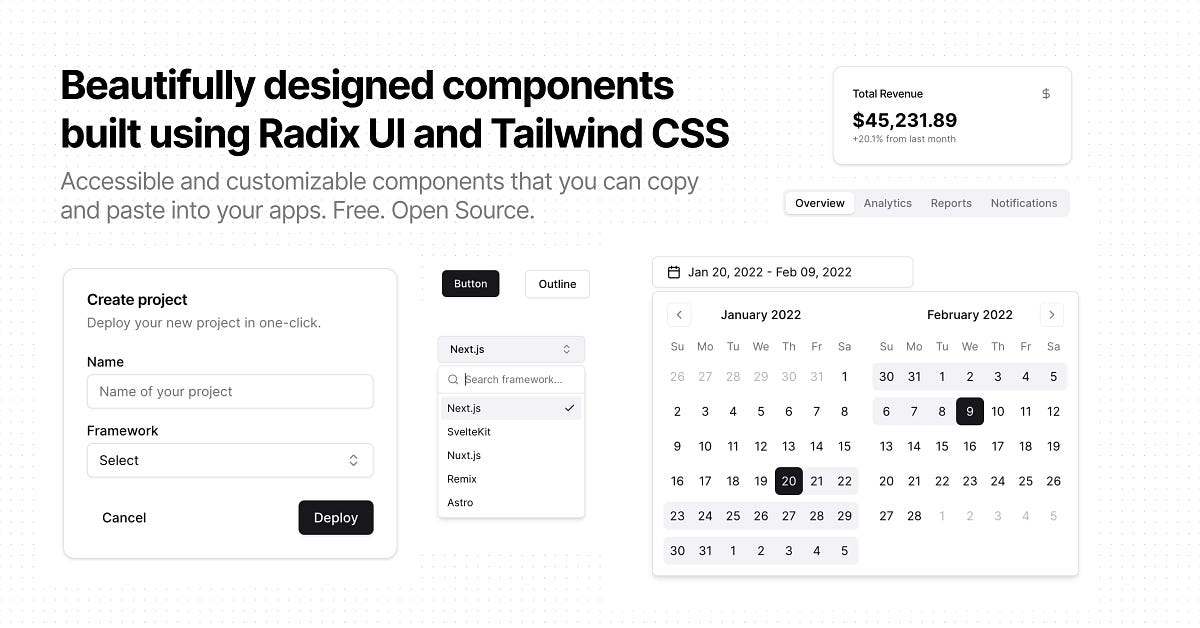
\includegraphics[width=0.85\textwidth,height=5.5cm,keepaspectratio]{technology/shadcnui.jpg}
    \caption{\textit{shadcn/ui --- component UI trên Radix UI và Tailwind CSS}}
    \label{fig:logo-shadcn}
\end{figure}

\subsubsection*{HugeIcons}
Thư viện icon \texttt{@hugeicons/react} cung cấp bộ icon phong phú và nhất quán về mặt thiết kế, được sử dụng xuyên suốt giao diện để cải thiện trải nghiệm người dùng.

\subsubsection*{Recharts và shadcn/chart}
Thư viện Recharts kết hợp với wrapper shadcn/chart được dùng để vẽ các biểu đồ thống kê trên dashboard nội bộ, bao gồm biểu đồ đường (Line Chart) theo dõi số đơn ứng tuyển, biểu đồ cột (Bar Chart) so sánh hiệu quả tuyển dụng theo kênh.

\subsection{Quản lý State và Data Fetching}

\subsubsection*{TanStack React Query v5}
React Query là giải pháp quản lý trạng thái dữ liệu bất đồng bộ (asynchronous data state) phía client. Hệ thống sử dụng React Query để:
\begin{itemize}
    \item \textbf{Caching thông minh:} Dữ liệu được lưu cache theo key, tránh gọi API trùng lặp. Ví dụ: dữ liệu danh sách jobs được cache 2 phút, thông tin user được cache 5 phút.
    \item \textbf{Background refetch:} Tự động làm mới dữ liệu khi người dùng quay lại tab.
    \item \textbf{Optimistic Updates:} Cập nhật UI ngay lập tức trước khi server xác nhận để trải nghiệm mượt mà hơn.
    \item \textbf{Error Handling:} Quản lý trạng thái loading, success, error một cách thống nhất.
    \item \textbf{DevTools:} Công cụ debug tích hợp, chỉ hiển thị trong môi trường development.
\end{itemize}

\begin{figure}[H]
    \centering
    
\includegraphics[width=0.72\textwidth,height=3.5cm,keepaspectratio]{technology/tanstack.png}
    \caption{\textit{TanStack Query --- cache và đồng bộ dữ liệu REST phía client}}
    \label{fig:logo-tanstack-query}
\end{figure}

\subsubsection*{TanStack React Table v8}
React Table (headless) được sử dụng để xây dựng các bảng dữ liệu phức tạp trong dashboard, hỗ trợ sắp xếp, lọc, phân trang và tùy biến hoàn toàn giao diện.

\subsection{Xử lý Form và Validation}

\subsubsection*{React Hook Form}
Thư viện xây dựng form hiệu suất cao, tránh re-render không cần thiết bằng cách sử dụng uncontrolled components. Kết hợp tốt với Zod để xác thực dữ liệu.

\subsubsection*{Zod}
Zod là thư viện schema validation cho TypeScript. Mỗi form và API endpoint đều có schema Zod riêng định nghĩa cấu trúc và quy tắc validate dữ liệu. Ưu điểm của Zod:
\begin{itemize}
    \item Type inference: Schema Zod tự động suy ra kiểu TypeScript tương ứng.
    \item Validation messages: Thông báo lỗi tùy biến bằng tiếng Việt.
    \item Transformations: Tự động chuyển đổi dữ liệu (ví dụ: trim whitespace, parse number).
\end{itemize}

\subsection{Cơ sở dữ liệu và ORM}

\subsubsection*{MariaDB / MySQL}
Hệ quản trị cơ sở dữ liệu quan hệ (RDBMS) được lựa chọn vì:
\begin{itemize}
    \item Phù hợp với mô hình dữ liệu có quan hệ chặt chẽ giữa các bảng (users, jobs, applications...).
    \item Hỗ trợ transaction ACID đảm bảo tính toàn vẹn dữ liệu.
    \item Hiệu suất cao với indexing và query optimization.
    \item Encoding utf8mb4 hỗ trợ đầy đủ tiếng Việt và emoji.
\end{itemize}

\subsubsection*{Prisma 7 ORM}
Prisma là ORM thế hệ mới cho TypeScript/JavaScript, mang lại:
\begin{itemize}
    \item \textbf{Type-safe queries:} Mọi query đều được kiểm tra kiểu dữ liệu tại thời điểm biên dịch.
    \item \textbf{Schema-first:} Cấu trúc database được định nghĩa trong file \texttt{schema.prisma}, từ đó Prisma generate client TypeScript phù hợp.
    \item \textbf{Migrations:} Quản lý thay đổi schema database có version control.
    \item \textbf{Driver Adapter:} Sử dụng \texttt{@prisma/adapter-mariadb} bắt buộc với Prisma 7 để kết nối MariaDB.
\end{itemize}

\begin{figure}[H]
    \centering
    
\includegraphics[width=0.62\textwidth,height=3.4cm,keepaspectratio]{technology/prisma.png}
    \caption{\textit{Prisma ORM --- schema-first, migrations và client kiểu an toàn}}
    \label{fig:logo-prisma}
\end{figure}

\subsection{Bảo mật và Xác thực}

\subsubsection*{JSON Web Token (JWT) với thư viện jose}
Thay vì sử dụng thư viện xác thực có sẵn như NextAuth, nhóm tự implement hệ thống JWT để hiểu sâu hơn về cơ chế bảo mật:
\begin{itemize}
    \item \textbf{Thuật toán HS256:} JWT được ký bằng khóa bí mật \texttt{AUTH\_SECRET} lưu trong biến môi trường.
    \item \textbf{Payload:} Token chứa \texttt{userId}, \texttt{email}, \texttt{fullName}, \texttt{role} để tránh query database mỗi lần cần thông tin user.
    \item \textbf{httpOnly Cookie:} Token được lưu trong cookie httpOnly, không thể truy cập bằng JavaScript phía client, chống XSS attacks.
    \item \textbf{SameSite=Lax:} Bảo vệ chống CSRF attacks trong hầu hết trường hợp.
    \item \textbf{Thời hạn:} Token hết hạn sau 7 ngày, yêu cầu đăng nhập lại.
\end{itemize}

\subsubsection*{Role-Based Access Control (RBAC)}
Hệ thống phân quyền dựa trên vai trò với 4 mức quyền hạn:
\begin{itemize}
    \item \textbf{candidate:} Truy cập \texttt{/candidate}, nộp đơn, quản lý hồ sơ cá nhân.
    \item \textbf{hr:} Truy cập \texttt{/dashboard}, quản lý jobs, applications, interviews.
    \item \textbf{admin:} Full access toàn hệ thống, quản lý tài khoản người dùng.
    \item \textbf{interviewer:} Xem lịch phỏng vấn được phân công và chấm điểm ứng viên.
\end{itemize}

\subsubsection*{bcrypt}
Mật khẩu người dùng được hash bằng thuật toán bcrypt với 12 salt rounds trước khi lưu vào database, đảm bảo an toàn ngay cả khi database bị tấn công.

\subsection{Dịch vụ bên thứ ba}

\begin{itemize}
    \item \textbf{Appwrite Storage:} Dịch vụ lưu trữ file đám mây dùng để lưu trữ CV và tài liệu của ứng viên, cung cấp URL truy cập an toàn.
    \item \textbf{Resend:} Dịch vụ gửi email transactional, được dùng để gửi OTP xác thực email và các thông báo cho ứng viên.
    \item \textbf{Sonner:} Thư viện Toast notification nhẹ, hiển thị thông báo thành công/lỗi cho người dùng.
\end{itemize}

\subsection{Tổng hợp Stack công nghệ}

\begin{table}[H]
    \centering
    \renewcommand{\arraystretch}{1.4}
    \begin{tabular}{|l|l|p{7cm}|}
        \hline
        \textbf{Lớp} & \textbf{Công nghệ} & \textbf{Ghi chú} \\ \hline
        Framework & Next.js 16 (App Router) & Server + Client Components \\ \hline
        Ngôn ngữ & TypeScript 5 & Strict mode \\ \hline
        Database & MariaDB / MySQL & Hosted riêng \\ \hline
        ORM & Prisma 7 & Driver adapter MariaDB \\ \hline
        Styling & Tailwind CSS 4 & Utility-first \\ \hline
        UI Components & shadcn/ui (Radix UI) & \texttt{components/ui/} \\ \hline
        Icons & @hugeicons/react & HugeIcons free set \\ \hline
        Form & React Hook Form + Zod & Schema-first validation \\ \hline
        Data Fetching & TanStack React Query v5 & Client-side caching \\ \hline
        Table & TanStack React Table v8 & Headless table \\ \hline
        Charts & Recharts + shadcn/chart & Biểu đồ dashboard \\ \hline
        Auth & JWT (HS256) với jose & httpOnly cookie, tự implement \\ \hline
        File Storage & Appwrite & CV và tài liệu upload \\ \hline
        Email & Resend & OTP và thông báo \\ \hline
        Toast & Sonner & Thông báo UX \\ \hline
        Fonts & Montserrat, Geist & Google Fonts + Vercel Fonts \\ \hline
    \end{tabular}
    \caption{\textit{Bảng tổng hợp công nghệ sử dụng trong hệ thống ATS}}
    \label{tab:tech_stack}
\end{table}


\section{KIẾN TRÚC HỆ THỐNG VÀ MÔ HÌNH DỮ LIỆU}
    \subsection{Sơ đồ kiến trúc hệ thống}
Hình~\ref{fig:ats-architecture} mô tả kiến trúc đa tầng của ATS: một ứng dụng Next.js~16 mono-repo làm điểm vào duy nhất cho giao diện và REST API; trạng thái phiên nằm trong cookie JWT (không lưu session DB); lưu trữ nghiệp vụ vào MariaDB qua Prisma; tích hợp các dịch vụ ngoài khi không cần trùng giá trị với lõi ATS.

\begin{figure}[H]
  \centering
  \begin{tikzpicture}[
      node distance=8mm,
      font=\footnotesize,
      >=Latex,
      box/.style={draw, rounded corners=3pt, inner sep=6pt,
        text width=0.86\linewidth, align=left},
      arr/.style={->, thick},
    ]
    % Ghi chu: nhan ky thuat trong node dung tieng Anh (tranh loi ma hoa font TikZ voi T5 khi viet tieng Viet trong node).
    \node[box] (L1) {\textbf{(1) Client (browser)}\\[1mm]
      React~19 --- Server + Client Components; Tailwind \& shadcn/ui; TanStack Query (REST cache/sync).};
    \node[box, below=of L1] (L2) {\textbf{(2) Next.js App Router --- same repository}\\[1mm]
      \texttt{app/*}: public jobs, dashboard, candidate, auth route-group;\\
      \texttt{app/api/**/*}: REST handlers (JSON envelope, Zod, bcrypt);\\
      \texttt{middleware.ts}: early RBAC gates; JWT in httpOnly cookie (\texttt{jose}, HS256).};
    \node[box, below=of L2] (L3) {\textbf{(3) Persistence}\\[1mm]
      Prisma~7 + MariaDB adapter --- schema-first ORM; transactions for invariant writes (applications + files metadata).};
    \node[box, below=of L3] (L4) {\textbf{(4) External adapters}\\[1mm]
      Appwrite Storage --- CV/binary blobs; Resend --- verification, invitations, transactional mail.};
    \draw[arr] (L1) -- (L2);
    \draw[arr] (L2) -- (L3);
    \draw[arr] (L3) -- (L4);
    % Outbound HTTPS from API tier to integrations (conceptual lateral hop)
    \draw[arr, dashed] (L2.east) to[bend left=25] (L4.east);
  \end{tikzpicture}
  \caption{\textit{Sơ đồ kiến trúc tổng thể ATS --- luồng yêu cầu và phân lớp trách nhiệm}}
  \label{fig:ats-architecture}
\end{figure}

\subsubsection*{Mô hình thiết kế:}
\begin{itemize}
    \item \textbf{Đơn codebase Next.js làm hai vai trò (UI + API):}
    Route Handlers cùng project với giao diện giảm độ trễ triển khai, chia sẻ kiểu TypeScript và tái dùng thư viện auth/validation; không buộc tách một service backend riêng --- phù hợp phạm vi dự án và nhóm phát triển nhỏ.

    \item \textbf{JWT trong cookie httpOnly + SameSite=Lax:}
    Tránh để token rơi vào JavaScript (giảm rủi ro XSS đọc trộm session); phía server chỉ đọc cookie và \texttt{verifySessionToken()}, không giữ phiên trong bảng \texttt{sessions} --- ít chỗ nhất quán phải ghi vào DB, dễ scale ngang và phù hợp SSR/Route Handlers.

    \item \textbf{MariaDB là nguồn sự thật duy nhất cho dữ liệu nghiệp vụ:}
    ATS xử lý quan hệ ứng viên--đơn--PV--tin tuyển dụng; Prisma đảm bảo migrate/schema rõ và truy vấn an toàn kiểu, phù hợp báo cáo và báo KPI.

    \item \textbf{Appwrite và Resend không lưu thay thế dữ liệu lõi:}
    File và email là các concern xâm nhập và tuân luật nhanh đổi; tách ra dịch vụ chuyên biệt cho phép giữ codebase HR mỏng, đổi nhà cung cấp mà không phải tái kiến trúc bảng ứng dụng.

    \item \textbf{TanStack Query ở client:}
    Chuẩn hóa cache, tái fetch và trạng thái đang tải cho các bảng long-poll không cần; Server Components dùng nơi ít interaction để SEO và giảm JS gửi trình duyệt.

\end{itemize}

\subsection{Cấu trúc thư mục dự án}
Hệ thống theo chuẩn App Router của Next.js, phân tách rõ vai trò từng thư mục:

\begin{itemize}
    \item \textbf{\texttt{app/}}: Chứa toàn bộ trang và API routes theo cấu trúc file-based routing.
    \begin{itemize}
        \item \textbf{\texttt{(auth)/}}: Route group cho đăng nhập, đăng ký, quên mật khẩu, xác minh email (không thêm segment vào URL).
        \item \textbf{\texttt{jobs/}}: Job portal công khai --- danh sách và chi tiết công việc.
        \item \textbf{\texttt{dashboard/}}: Khu vực nội bộ dành cho Admin, HR, Interviewer.
        \item \textbf{\texttt{candidate/}}: Khu vực riêng của ứng viên.
        \item \textbf{\texttt{api/}}: Toàn bộ Route Handlers (REST API).
    \end{itemize}
    \item \textbf{\texttt{components/}}: Các thành phần UI tái sử dụng (auth, landing, providers, shadcn/ui).
    \item \textbf{\texttt{hooks/}}: Custom hooks tích hợp React Query cho mọi endpoint.
    \item \textbf{\texttt{lib/}}: Các tiện ích dùng chung --- cấu hình DB, xử lý HTTP, JWT, validators.
    \item \textbf{\texttt{prisma/}}: Schema mô hình dữ liệu và seed data mẫu.
    \item \textbf{\texttt{types/}}: Các kiểu TypeScript dùng chung (ApiSuccess, ApiErrorBody, PublicUser).
\end{itemize}

\subsection{Phân quyền theo Role (RBAC)}

\begin{table}[H]
    \centering
    \renewcommand{\arraystretch}{1.4}
    \begin{tabular}{|l|p{9cm}|}
        \hline
        \textbf{Route} & \textbf{Quyền truy cập} \\ \hline
        \texttt{/} · \texttt{/jobs} · \texttt{/jobs/[slug]} & Tất cả (public, không cần đăng nhập) \\ \hline
        \texttt{/login} · \texttt{/register} & Chỉ khách chưa đăng nhập \\ \hline
        \texttt{/candidate} & Role: \texttt{candidate} \\ \hline
        \texttt{/dashboard} và sub-routes & Role: \texttt{admin}, \texttt{hr}, \texttt{interviewer} \\ \hline
        \texttt{/unauthorized} & Fallback khi truy cập sai role \\ \hline
    \end{tabular}
    \caption{\textit{Bảng phân quyền theo route}}
    \label{tab:rbac}
\end{table}

\subsection{Mô hình dữ liệu (Data Model)}
Cơ sở dữ liệu của hệ thống ATS bao gồm 11 bảng chính:

\subsubsection*{1. Bảng \texttt{users} (Tài khoản người dùng)}
\begin{itemize}
    \item \textbf{\texttt{id}}: Khóa chính (UUID).
    \item \textbf{\texttt{email}}: Email đăng nhập (Unique).
    \item \textbf{\texttt{password\_hash}}: Mật khẩu đã mã hóa bcrypt (null nếu OAuth).
    \item \textbf{\texttt{full\_name}, \texttt{phone}, \texttt{avatar\_url}}: Thông tin cá nhân.
    \item \textbf{\texttt{role}}: Phân quyền --- \texttt{candidate | admin | hr | interviewer}.
    \item \textbf{\texttt{provider}}: Phương thức đăng nhập (\texttt{local} hoặc OAuth provider).
    \item \textbf{\texttt{is\_active}}: Cờ kích hoạt tài khoản (boolean).
    \item \textbf{\texttt{email\_verified}}: Trạng thái xác minh email (boolean).
    \item \textbf{\texttt{last\_login\_at}, \texttt{created\_at}, \texttt{updated\_at}}: Các mốc thời gian.
\end{itemize}

\subsubsection*{2. Bảng \texttt{otp\_tokens} (Mã xác thực OTP)}
\begin{itemize}
    \item \textbf{\texttt{id}, \texttt{email}}: Khóa chính (UUID) và email nhận mã.
    \item \textbf{\texttt{code}}: Chuỗi OTP 6 ký tự số (có thể được hash).
    \item \textbf{\texttt{type}}: Loại OTP --- \texttt{email\_verify} hoặc \texttt{password\_reset}.
    \item \textbf{\texttt{attempts}}: Số lần nhập sai (tối đa giới hạn trước khi vô hiệu).
    \item \textbf{\texttt{expires\_at}}: Thời điểm hết hạn (15 phút kể từ khi tạo).
    \item \textbf{\texttt{used\_at}}: Thời điểm đã sử dụng (null = chưa dùng).
\end{itemize}

\subsubsection*{3. Bảng \texttt{candidate\_profiles} (Hồ sơ ứng viên)}
Quan hệ 1-1 với \texttt{users}, chứa thông tin nghề nghiệp chi tiết:
\begin{itemize}
    \item \textbf{\texttt{user\_id}}: Khóa ngoại (Unique) liên kết tới \texttt{users}.
    \item \textbf{\texttt{title}, \texttt{bio}, \texttt{location}}: Chức danh, giới thiệu, địa điểm.
    \item \textbf{\texttt{years\_experience}}: Số năm kinh nghiệm.
    \item \textbf{\texttt{skills}, \texttt{education}}: Kỹ năng và học vấn (lưu dạng JSON array).
    \item \textbf{\texttt{linkedin\_url}, \texttt{github\_url}}: Liên kết mạng xã hội nghề nghiệp.
\end{itemize}

\subsubsection*{4. Bảng \texttt{files} (Tệp tin đính kèm)}
\begin{itemize}
    \item \textbf{\texttt{user\_id}}: Khóa ngoại tới chủ sở hữu file.
    \item \textbf{\texttt{file\_name}, \texttt{file\_url}}: Tên gốc và URL lưu trữ (Appwrite).
    \item \textbf{\texttt{file\_type}}: Phân loại --- \texttt{cv}, \texttt{portfolio}, \texttt{certificate}.
    \item \textbf{\texttt{appwrite\_id}}: ID file trên Appwrite Storage.
\end{itemize}

\subsubsection*{5. Bảng \texttt{jobs} (Tin tuyển dụng)}
\begin{itemize}
    \item \textbf{\texttt{created\_by}}: Khóa ngoại tới HR/Admin tạo tin.
    \item \textbf{\texttt{title}, \texttt{slug}}: Tiêu đề và định danh URL (đều Unique).
    \item \textbf{\texttt{description}, \texttt{requirements}, \texttt{benefits}}: Nội dung mô tả việc làm.
    \item \textbf{\texttt{location}, \texttt{department}, \texttt{category}}: Phân loại công việc.
    \item \textbf{\texttt{salary\_min}, \texttt{salary\_max}}: Khoảng lương (VND).
    \item \textbf{\texttt{employment\_type}}: Loại hợp đồng --- \texttt{full\_time | part\_time | contract}.
    \item \textbf{\texttt{required\_skills}}: Mảng kỹ năng yêu cầu (JSON).
    \item \textbf{\texttt{headcount}}: Số lượng vị trí cần tuyển.
    \item \textbf{\texttt{status}}: Trạng thái --- \texttt{draft | active | closed | archived}.
    \item \textbf{\texttt{expires\_at}, \texttt{published\_at}}: Thời hạn và ngày đăng công khai.
\end{itemize}

\subsubsection*{6. Bảng \texttt{job\_channels} (Kênh phân phối tin)}
\begin{itemize}
    \item \textbf{\texttt{job\_id}}: Khóa ngoại tới \texttt{jobs}.
    \item \textbf{\texttt{channel}}: Nền tảng đăng tin --- \texttt{linkedin | itviec | topcv | vietnamworks | website}.
    \item \textbf{\texttt{external\_url}, \texttt{external\_id}}: URL bài đăng ngoài và ID trên kênh đó.
    \item \textbf{\texttt{status}}: Trạng thái --- \texttt{pending | posted | failed | expired | removed}.
    \item \textbf{\texttt{posted\_at}, \texttt{expires\_at}, \texttt{error\_message}}: Thông tin đăng và lỗi (nếu có).
\end{itemize}
\textit{Ràng buộc Unique: \texttt{(job\_id, channel)} --- mỗi kênh chỉ đăng một lần cho mỗi tin.}

\subsubsection*{7. Bảng \texttt{applications} (Đơn ứng tuyển)}
\begin{itemize}
    \item \textbf{\texttt{job\_id}, \texttt{candidate\_id}}: Khóa ngoại tới công việc và ứng viên.
    \item \textbf{\texttt{cv\_file\_url}, \texttt{cv\_filename}}: Đường dẫn và tên file CV.
    \item \textbf{\texttt{cover\_letter}}: Thư giới thiệu (tùy chọn).
    \item \textbf{\texttt{status}}: Vòng đời --- \texttt{applied} $\to$ \texttt{screening} $\to$ \texttt{interviewing} $\to$ \texttt{offered} $\to$ \texttt{hired} hoặc \texttt{rejected}.
    \item \textbf{\texttt{source\_channel}}: Nguồn nhận đơn (VD: từ linkedin, website...).
    \item \textbf{\texttt{applied\_at}}: Thời điểm nộp đơn.
\end{itemize}
\textit{Ràng buộc Unique: \texttt{(job\_id, candidate\_id)} --- mỗi ứng viên chỉ nộp một đơn cho mỗi job.}

\subsubsection*{8. Bảng \texttt{application\_status\_history} (Lịch sử trạng thái)}
\begin{itemize}
    \item \textbf{\texttt{application\_id}, \texttt{changed\_by}}: Tham chiếu đơn và người thay đổi (HR/Admin).
    \item \textbf{\texttt{from\_status}, \texttt{to\_status}}: Trạng thái cũ và mới.
    \item \textbf{\texttt{note}}: Ghi chú lý do thay đổi.
    \item \textbf{\texttt{changed\_at}}: Thời điểm thay đổi.
\end{itemize}

\subsubsection*{9. Bảng \texttt{email\_logs} (Nhật ký email)}
\begin{itemize}
    \item \textbf{\texttt{application\_id}, \texttt{recipient\_id}, \texttt{sender\_id}}: Các tham chiếu liên quan.
    \item \textbf{\texttt{subject}}: Tiêu đề email.
    \item \textbf{\texttt{type}}: Phân loại --- \texttt{invite | result | reminder | rejection | offer}.
    \item \textbf{\texttt{status}}: Kết quả gửi --- \texttt{pending | sent | failed}.
    \item \textbf{\texttt{sent\_at}, \texttt{error\_message}}: Thời điểm gửi và thông báo lỗi nếu có.
\end{itemize}

\subsubsection*{10. Bảng \texttt{interviews} (Lịch phỏng vấn)}
\begin{itemize}
    \item \textbf{\texttt{application\_id}, \texttt{interviewer\_id}}: Tham chiếu đơn và người phỏng vấn.
    \item \textbf{\texttt{scheduled\_at}}: Ngày giờ phỏng vấn.
    \item \textbf{\texttt{duration\_minutes}}: Thời lượng (mặc định 60 phút).
    \item \textbf{\texttt{type}}: Hình thức --- \texttt{phone | video | onsite | technical}.
    \item \textbf{\texttt{status}}: Trạng thái --- \texttt{scheduled | completed | cancelled | rescheduled}.
    \item \textbf{\texttt{meeting\_link}}: Link họp video (Zoom, Google Meet...).
    \item \textbf{\texttt{location}}: Địa điểm (cho phỏng vấn trực tiếp).
    \item \textbf{\texttt{notes}}: Ghi chú hướng dẫn cho ứng viên.
\end{itemize}

\subsubsection*{11. Bảng \texttt{interview\_scores} (Điểm đánh giá phỏng vấn)}
\begin{itemize}
    \item \textbf{\texttt{interview\_id}, \texttt{evaluator\_id}}: Tham chiếu buổi phỏng vấn và người chấm điểm.
    \item \textbf{\texttt{technical\_score}}: Điểm kỹ thuật (thang 1--10).
    \item \textbf{\texttt{communication\_score}}: Điểm giao tiếp (thang 1--10).
    \item \textbf{\texttt{cultural\_fit\_score}}: Điểm phù hợp văn hóa (thang 1--10).
    \item \textbf{\texttt{overall\_score}}: Điểm tổng thể (thang 1--10).
    \item \textbf{\texttt{strengths}, \texttt{weaknesses}, \texttt{feedback}}: Nhận xét tự luận.
    \item \textbf{\texttt{result}}: Quyết định cuối --- \texttt{pass | fail | hold}.
    \item \textbf{\texttt{is\_final}}: Cờ chốt điểm, khi \texttt{true} sẽ cập nhật trạng thái interview thành \texttt{completed}.
\end{itemize}
\textit{Dùng pattern UPSERT theo \texttt{(interview\_id, evaluator\_id)} --- cập nhật thay vì tạo mới khi chấm lại.}

\subsection{Sơ đồ quan hệ thực thể (ERD)}

\begin{table}[H]
    \centering
    \renewcommand{\arraystretch}{1.4}
    \begin{tabular}{|l|c|l|l|}
        \hline
        \textbf{Bảng cha} & \textbf{Quan hệ} & \textbf{Bảng con} & \textbf{Khóa ngoại} \\ \hline
        \texttt{users} & 1 -- 1 & \texttt{candidate\_profiles} & \texttt{user\_id} \\ \hline
        \texttt{users} & 1 -- N & \texttt{files} & \texttt{user\_id} \\ \hline
        \texttt{users} & 1 -- N & \texttt{jobs} & \texttt{created\_by} \\ \hline
        \texttt{users} & 1 -- N & \texttt{applications} & \texttt{candidate\_id} \\ \hline
        \texttt{users} & 1 -- N & \texttt{email\_logs} & \texttt{recipient\_id / sender\_id} \\ \hline
        \texttt{users} & 1 -- N & \texttt{interviews} & \texttt{interviewer\_id} \\ \hline
        \texttt{users} & 1 -- N & \texttt{interview\_scores} & \texttt{evaluator\_id} \\ \hline
        \texttt{jobs} & 1 -- N & \texttt{job\_channels} & \texttt{job\_id} \\ \hline
        \texttt{jobs} & 1 -- N & \texttt{applications} & \texttt{job\_id} \\ \hline
        \texttt{applications} & 1 -- N & \texttt{application\_status\_history} & \texttt{application\_id} \\ \hline
        \texttt{applications} & 1 -- N & \texttt{email\_logs} & \texttt{application\_id} \\ \hline
        \texttt{applications} & 1 -- N & \texttt{interviews} & \texttt{application\_id} \\ \hline
        \texttt{interviews} & 1 -- N & \texttt{interview\_scores} & \texttt{interview\_id} \\ \hline
    \end{tabular}
    \caption{\textit{Sơ đồ quan hệ giữa các bảng trong hệ thống ATS}}
    \label{tab:erd}
\end{table}

\subsection{Chiến lược Caching với React Query}

\begin{table}[H]
    \centering
    \renewcommand{\arraystretch}{1.4}
    \begin{tabular}{|l|l|l|l|}
        \hline
        \textbf{Hook} & \textbf{Endpoint} & \textbf{staleTime} & \textbf{Retry} \\ \hline
        \texttt{useMe()} & \texttt{GET /api/auth/me} & 5 phút & false (không retry 401) \\ \hline
        \texttt{useJobs()} & \texttt{GET /api/jobs} & 2 phút & Mặc định \\ \hline
        \texttt{useJob(slug)} & \texttt{GET /api/jobs/[slug]} & 5 phút & false khi 404/401 \\ \hline
    \end{tabular}
    \caption{\textit{Chiến lược caching của React Query}}
    \label{tab:caching}
\end{table}

Cấu hình \texttt{refetchOnWindowFocus: false} được áp dụng toàn cục để tắt tính năng refetch tự động khi người dùng chuyển tab, tránh các request thừa không cần thiết.


\section{THIẾT KẾ CHỨC NĂNG THEO MODULE}
    % Ảnh giao diện: report/image/ (cùng cấu trúc A/1.png … G/4.png); đường tìm trong main.tex qua \graphicspath{{./image/}}
\providecommand{\FigDDCaption}[3]{%
  \begin{figure}[H]
    \centering
    \includegraphics[width=\linewidth,height=0.88\textheight,keepaspectratio]{#1/#2.png}
    \caption{\textit{#3}}
  \end{figure}%
}

Hệ thống ATS được tổ chức thành 7 module chức năng, mỗi module đảm nhiệm một nhóm nghiệp vụ riêng biệt và phục vụ các đối tượng người dùng khác nhau.

\subsection{Module A --- Khu vực Công khai (Public \& Landing)}
\textbf{Người phụ trách:} Vương Quang Khải

\subsubsection*{Danh sách chức năng}
\begin{table}[H]
    \centering
    \renewcommand{\arraystretch}{1.3}
    \begin{tabular}{|c|l|l|l|}
        \hline
        \textbf{STT} & \textbf{Chức năng} & \textbf{Route} & \textbf{Quyền} \\ \hline
        1 & Trang chủ (Landing Page) & \texttt{/} & Public \\ \hline
        2 & Danh sách việc làm & \texttt{/jobs} & Public \\ \hline
        3 & Chi tiết việc làm & \texttt{/jobs/[slug]} & Public \\ \hline
        4 & Nộp đơn ứng tuyển & \texttt{POST /api/jobs/[slug]/apply} & Candidate \\ \hline
    \end{tabular}
    \caption{\textit{Danh sách chức năng Module A}}
\end{table}

\subsubsection*{Mô tả chức năng}
\textbf{Trang chủ (Landing Page)} hiển thị hero section giới thiệu hệ thống, tối đa 6 tin tuyển dụng nổi bật (\texttt{status = active}), sắp xếp theo ngày tạo mới nhất. Khi chưa đăng nhập, hiển thị nút CTA ``Đăng nhập'' và ``Đăng ký''; khi đã đăng nhập hiển thị UserNav với avatar và dropdown menu.

\textbf{Danh sách việc làm} là Client Component sử dụng React Query để fetch và cache dữ liệu. Hỗ trợ tìm kiếm và lọc đa tiêu chí: từ khóa (keyword), địa điểm (location), loại hợp đồng (employment\_type), phòng ban (department). Các tham số lọc được đồng bộ với URL query string để có thể chia sẻ link kết quả tìm kiếm.

\textbf{Chi tiết việc làm} hiển thị đầy đủ thông tin job, danh sách kênh đăng tuyển bên ngoài (job\_channels với status = posted). Kiểm tra trạng thái ứng tuyển của candidate đang đăng nhập: nếu đã nộp $\to$ hiển thị badge ``Đã ứng tuyển'', nếu chưa $\to$ hiển thị nút ``Ứng tuyển ngay''.

\textbf{Form nộp đơn} (modal overlay) yêu cầu candidate upload file CV (PDF/DOC/DOCX, tối đa 5MB) và nhập thư giới thiệu (tùy chọn, tối đa 2000 ký tự). CV được upload lên Appwrite Storage, sau đó tạo record trong bảng \texttt{applications} và \texttt{files} trong một transaction.

\subsubsection*{Các API của Module A}
\begin{table}[H]
    \centering
    \renewcommand{\arraystretch}{1.3}
    \begin{tabular}{|c|l|l|p{5cm}|}
        \hline
        \textbf{Method} & \textbf{Endpoint} & \textbf{Auth} & \textbf{Mô tả} \\ \hline
        GET & \texttt{/api/jobs} & Public & Danh sách jobs active, hỗ trợ filter \\ \hline
        GET & \texttt{/api/jobs/[slug]} & Public & Chi tiết job + job\_channels \\ \hline
        POST & \texttt{/api/jobs/[slug]/apply} & Candidate & Tạo đơn ứng tuyển, upload CV \\ \hline
    \end{tabular}
    \caption{\textit{Danh sách API Module A}}
\end{table}

\subsubsection*{Thông báo hệ thống (Module A)}
\begin{table}[H]
    \centering
    \renewcommand{\arraystretch}{1.3}
    \begin{tabular}{|l|l|p{8cm}|}
        \hline
        \textbf{Mã} & \textbf{Loại} & \textbf{Nội dung} \\ \hline
        MSG-A-001 & Success & Nộp đơn thành công! Chúng tôi sẽ liên hệ với bạn sớm. \\ \hline
        MSG-A-002 & Error & Không tìm thấy việc làm này hoặc việc làm đã đóng. \\ \hline
        MSG-A-004 & Warning & Bạn đã nộp đơn cho vị trí này trước đó. \\ \hline
        MSG-A-006 & Validation & Vui lòng tải lên file CV định dạng PDF, DOC hoặc DOCX. \\ \hline
        MSG-A-007 & Validation & File CV không được vượt quá 5MB. \\ \hline
    \end{tabular}
    \caption{\textit{Danh sách thông báo Module A}}
\end{table}

\subsubsection*{Minh họa giao diện}
\FigDDCaption{A}{1}{Module A --- Trang chủ}
\FigDDCaption{A}{2}{Module A --- Trang danh sách việc làm}
\FigDDCaption{A}{3}{Module A --- Trang chi tiết việc làm}
\FigDDCaption{A}{4}{Module A --- Modal nộp đơn ứng tuyển}

\subsection{Module B --- Xác thực (Authentication)}
\textbf{Người phụ trách:} Lê Huỳnh Huy

\subsubsection*{Danh sách chức năng}
\begin{table}[H]
    \centering
    \renewcommand{\arraystretch}{1.3}
    \begin{tabular}{|c|l|l|}
        \hline
        \textbf{STT} & \textbf{Chức năng} & \textbf{Route} \\ \hline
        1 & Đăng nhập & \texttt{/(auth)/login} \\ \hline
        2 & Đăng ký & \texttt{/(auth)/register} \\ \hline
        3 & Quên mật khẩu (gửi OTP reset) & \texttt{/(auth)/forgot-password} \\ \hline
        4 & Xác minh email bằng OTP & \texttt{/(auth)/verify-email} \\ \hline
        5 & Đăng xuất & \texttt{POST /api/auth/logout} \\ \hline
        6 & Lấy thông tin user hiện tại & \texttt{GET /api/auth/me} \\ \hline
        7 & Đổi mật khẩu & \texttt{POST /api/auth/password} \\ \hline
    \end{tabular}
    \caption{\textit{Danh sách chức năng Module B}}
\end{table}

\subsubsection*{Luồng xử lý Đăng nhập}
\begin{enumerate}
    \item Validate Zod schema: email format, password không rỗng.
    \item Tra cứu user theo email từ database.
    \item Kiểm tra \texttt{is\_active = true} (nếu false $\to$ 403 tài khoản bị khóa).
    \item So sánh password với \texttt{bcrypt.compare(password, password\_hash)}.
    \item Ký JWT HS256 (\texttt{signSessionToken}), hết hạn sau 7 ngày.
    \item Set httpOnly cookie: \texttt{session=<jwt>; HttpOnly; SameSite=Lax; Max-Age=604800}.
    \item Cập nhật \texttt{last\_login\_at} (fire-and-forget, không block response).
    \item Trả về PublicUser (không bao gồm password\_hash).
    \item Client-side redirect theo role: candidate $\to$ \texttt{/candidate}, admin/hr/interviewer $\to$ \texttt{/dashboard}.
\end{enumerate}

\subsubsection*{Luồng xử lý Đăng ký}
\begin{enumerate}
    \item Validate Zod: email hợp lệ, password $\ge$ 8 ký tự, fullName không rỗng.
    \item Kiểm tra email trùng lặp (\texttt{findUnique WHERE email}).
    \item Hash password: \texttt{bcrypt.hash(password, 12)} (12 salt rounds).
    \item Tạo user với \texttt{role = 'candidate'}, \texttt{email\_verified = false}.
    \item Tạo OTP 6 số ngẫu nhiên, hết hạn sau 15 phút, type = \texttt{email\_verify}.
    \item Lưu OTP vào bảng \texttt{otp\_tokens}.
    \item Gửi email qua Resend API với template xác minh.
    \item Redirect đến trang \texttt{/verify-email} để nhập OTP.
\end{enumerate}

\subsubsection*{Quy tắc validation form Đăng ký}
\begin{table}[H]
    \centering
    \renewcommand{\arraystretch}{1.3}
    \begin{tabular}{|c|l|l|l|}
        \hline
        \textbf{STT} & \textbf{Trường} & \textbf{Điều kiện} & \textbf{Thông báo lỗi} \\ \hline
        1 & Họ và tên & Bắt buộc, 2--100 ký tự & MSG-B-008 \\ \hline
        2 & Email & Bắt buộc, định dạng hợp lệ & MSG-B-005 \\ \hline
        3 & Số điện thoại & Tùy chọn; 10--15 chữ số & --- \\ \hline
        4 & Mật khẩu & Bắt buộc, tối thiểu 8 ký tự & MSG-B-006 \\ \hline
        5 & Xác nhận mật khẩu & Phải khớp với mật khẩu & MSG-B-010 \\ \hline
    \end{tabular}
    \caption{\textit{Quy tắc validation form Đăng ký}}
\end{table}

\subsubsection*{Các API của Module B}
\begin{table}[H]
    \centering
    \renewcommand{\arraystretch}{1.3}
    \begin{tabular}{|c|l|l|l|}
        \hline
        \textbf{No} & \textbf{Method} & \textbf{Endpoint} & \textbf{Mô tả} \\ \hline
        1 & POST & \texttt{/api/auth/login} & Đăng nhập, phát JWT cookie \\ \hline
        2 & POST & \texttt{/api/auth/register} & Tạo user + gửi OTP xác minh \\ \hline
        3 & POST & \texttt{/api/auth/logout} & Xóa session cookie \\ \hline
        4 & POST & \texttt{/api/auth/otp/send} & Gửi OTP (xác minh / reset) \\ \hline
        5 & POST & \texttt{/api/auth/otp/verify-email} & Kích hoạt tài khoản bằng OTP \\ \hline
        6 & POST & \texttt{/api/auth/otp/reset-password} & Đặt lại mật khẩu bằng OTP \\ \hline
        7 & GET & \texttt{/api/auth/me} & Thông tin user đang đăng nhập \\ \hline
        8 & POST & \texttt{/api/auth/password} & Đổi mật khẩu khi đã đăng nhập \\ \hline
    \end{tabular}
    \caption{\textit{Danh sách API Module B}}
\end{table}

\subsubsection*{Minh họa giao diện}
\FigDDCaption{B}{1}{Module B --- Trang đăng nhập}
\FigDDCaption{B}{2}{Module B --- Trang đăng ký}
\FigDDCaption{B}{3}{Module B --- Quên mật khẩu --- bước 1}
\FigDDCaption{B}{4}{Module B --- Quên mật khẩu --- gửi email}
\FigDDCaption{B}{5}{Module B --- Quên mật khẩu --- bước 2}

\subsection{Module C --- Khu vực Ứng viên (Candidate Area)}
\textbf{Người phụ trách:} Nguyễn Quang Sáng

Module C tập trung toàn bộ chức năng của ứng viên trong \textbf{một trang duy nhất} \texttt{/candidate} với bố cục 3 Tab, không có sub-route.

\subsubsection*{Cấu trúc 3 Tab}
\begin{table}[H]
    \centering
    \renewcommand{\arraystretch}{1.3}
    \begin{tabular}{|c|l|p{9cm}|}
        \hline
        \textbf{Tab} & \textbf{Tên hiển thị} & \textbf{Mô tả} \\ \hline
        1 & Đơn ứng tuyển & Danh sách đơn đã nộp với badge trạng thái, link CV, link đến job \\ \hline
        2 & Lịch phỏng vấn & Lịch phỏng vấn do HR lên, hiển thị ngày giờ, hình thức, link tham gia \\ \hline
        3 & Hồ sơ cá nhân & Xem/chỉnh sửa thông tin; đổi mật khẩu; xác minh email; quản lý file CV \\ \hline
    \end{tabular}
    \caption{\textit{Cấu trúc 3 Tab của Module C}}
\end{table}

\subsubsection*{Chức năng Tab Đơn ứng tuyển}
Hiển thị danh sách tất cả các đơn ứng tuyển của candidate, sắp xếp theo thời gian nộp mới nhất. Mỗi thẻ (card) hiển thị: tên vị trí (link đến /jobs/[slug]), ngày ứng tuyển, badge trạng thái (applied/screening/interviewing/offered/hired/rejected), link tải CV và thư giới thiệu.

\subsubsection*{Chức năng Tab Lịch phỏng vấn}
Hiển thị tất cả lịch phỏng vấn do HR tạo, liên kết với các đơn của candidate. Thông tin hiển thị bao gồm: vị trí phỏng vấn, thời gian (định dạng tiếng Việt), hình thức (Video/Điện thoại/Trực tiếp/Technical), thời lượng, link họp trực tuyến và ghi chú của HR.

\subsubsection*{Chức năng Tab Hồ sơ cá nhân}
\begin{itemize}
    \item \textbf{Xem/Chỉnh sửa hồ sơ:} Cập nhật thông tin cơ bản (họ tên, email, điện thoại), thông tin nghề nghiệp (chức danh, bio, địa điểm, số năm kinh nghiệm), liên kết mạng xã hội (LinkedIn, GitHub).
    \item \textbf{Đổi mật khẩu:} Xác nhận mật khẩu cũ, nhập và xác nhận mật khẩu mới (tối thiểu 8 ký tự).
    \item \textbf{Xác minh email OTP:} Gửi OTP qua email, nhập mã 6 số để kích hoạt badge xác minh. Tính năng cooldown 60 giây sau mỗi lần gửi.
    \item \textbf{Quản lý file CV:} Upload file (PDF/DOC/DOCX, $\le$ 5MB) lên Appwrite, đổi tên, xóa file khỏi hệ thống.
\end{itemize}

\subsubsection*{Danh sách API Module C}
\begin{table}[H]
    \centering
    \renewcommand{\arraystretch}{1.3}
    \begin{tabular}{|c|l|l|l|}
        \hline
        \textbf{No} & \textbf{Method} & \textbf{Endpoint} & \textbf{Mô tả} \\ \hline
        C-01 & GET & \texttt{/api/candidate/applications} & Danh sách đơn ứng tuyển \\ \hline
        C-02 & GET & \texttt{/api/candidate/interviews} & Danh sách lịch phỏng vấn \\ \hline
        C-03 & GET & \texttt{/api/candidate/profile} & Đọc hồ sơ + thông tin user \\ \hline
        C-04 & POST & \texttt{/api/candidate/profile} & Cập nhật hồ sơ, refresh JWT \\ \hline
        C-05 & PATCH & \texttt{/api/auth/password} & Đổi mật khẩu \\ \hline
        C-08 & GET & \texttt{/api/candidate/files} & Danh sách file cá nhân \\ \hline
        C-09 & POST & \texttt{/api/candidate/files} & Upload metadata file \\ \hline
        C-10 & PUT & \texttt{/api/candidate/files/[id]} & Đổi tên file \\ \hline
        C-11 & DELETE & \texttt{/api/candidate/files/[id]} & Xóa file \\ \hline
    \end{tabular}
    \caption{\textit{Danh sách API Module C}}
\end{table}

\subsubsection*{Minh họa giao diện}
\FigDDCaption{C}{1}{Module C --- Không gian ứng viên, tab đơn ứng tuyển}
\FigDDCaption{C}{2}{Module C --- Không gian ứng viên, tab lịch phỏng vấn}
\FigDDCaption{C}{3}{Module C --- Không gian ứng viên, tab hồ sơ cá nhân}

\subsection{Module D --- Quản trị nội bộ (Dashboard)}
\textbf{Người phụ trách:} Nguyễn Minh Khôi

Dashboard là trang tổng quan dành cho Admin, HR và Interviewer, hiển thị các chỉ số KPI quan trọng:
\begin{itemize}
    \item Tổng số tin tuyển dụng đang hoạt động.
    \item Số đơn ứng tuyển mới trong tuần/tháng.
    \item Số buổi phỏng vấn sắp diễn ra.
    \item Biểu đồ đường theo dõi xu hướng ứng tuyển theo thời gian.
    \item Biểu đồ cột so sánh hiệu quả các kênh đăng tuyển.
\end{itemize}

Module D cũng bao gồm trang quản lý tài khoản người dùng (\texttt{/admin/users}) dành riêng cho Admin: xem danh sách, lọc theo role, bật/tắt tài khoản, và hỗ trợ reset mật khẩu.

\subsubsection*{Minh họa giao diện}
\FigDDCaption{D}{1}{Module D --- Trang Dashboard}
\FigDDCaption{D}{2}{Module D --- Trang quản lý emails}

\subsection{Module E --- Quản lý Đơn ứng tuyển (Applications)}
\textbf{Người phụ trách:} Lê Đức Anh Tuấn

\subsubsection*{Danh sách chức năng}
\begin{itemize}
    \item \textbf{Pipeline tuyển dụng:} Hiển thị tất cả đơn ứng tuyển dưới dạng danh sách hoặc Kanban board, hỗ trợ lọc theo job, trạng thái, nguồn (source\_channel).
    \item \textbf{Chi tiết đơn ứng tuyển:} Xem đầy đủ hồ sơ ứng viên, lịch sử thay đổi trạng thái, danh sách buổi phỏng vấn và email đã gửi.
    \item \textbf{Cập nhật trạng thái:} Chuyển trạng thái đơn qua các bước pipeline, ghi chú lý do (lưu vào \texttt{application\_status\_history}).
    \item \textbf{Xem CV:} Tải xuống hoặc xem trực tiếp file CV của ứng viên.
\end{itemize}

\subsubsection*{Vòng đời trạng thái đơn ứng tuyển}

Trạng thái của mỗi đơn ứng tuyển tuân theo quy trình tuyến tính với khả năng từ chối ở bất kỳ bước nào:

\begin{center}
    \texttt{applied} $\to$ \texttt{screening} $\to$ \texttt{interviewing} $\to$ \texttt{offered} $\to$ \texttt{hired}\\
    \hspace{5cm} \texttt{rejected} (từ bất kỳ bước nào)
\end{center}

\begin{table}[H]
    \centering
    \renewcommand{\arraystretch}{1.3}
    \begin{tabular}{|l|l|l|}
        \hline
        \textbf{Trạng thái} & \textbf{Ý nghĩa} & \textbf{Bước tiếp theo} \\ \hline
        applied & Vừa nộp đơn & screening hoặc rejected \\ \hline
        screening & Đang sàng lọc hồ sơ & interviewing hoặc rejected \\ \hline
        interviewing & Đang trong quá trình phỏng vấn & offered hoặc rejected \\ \hline
        offered & Đã nhận được lời mời & hired hoặc rejected \\ \hline
        hired & Đã được tuyển dụng & Kết thúc \\ \hline
        rejected & Bị từ chối & Kết thúc \\ \hline
    \end{tabular}
    \caption{\textit{Vòng đời trạng thái đơn ứng tuyển}}
\end{table}

\subsubsection*{Minh họa giao diện}
\FigDDCaption{E}{1}{Module E --- Trang quản lý đơn ứng tuyển}
\FigDDCaption{E}{2}{Module E --- Chi tiết đơn --- tab lịch sử trạng thái}
\FigDDCaption{E}{3}{Module E --- Chi tiết đơn --- tab phỏng vấn}
\FigDDCaption{E}{4}{Module E --- Chi tiết đơn --- tab nhật ký email}
\FigDDCaption{E}{5}{Module E --- Form đổi trạng thái đơn}
\FigDDCaption{E}{6}{Module E --- Form lên lịch phỏng vấn}
\FigDDCaption{E}{7}{Module E --- Form gửi email}

\subsection{Module F --- Quản lý Phỏng vấn (Interviews)}
\textbf{Người phụ trách:} Bùi Minh Khôi

\subsubsection*{Danh sách chức năng}
\begin{itemize}
    \item \textbf{Danh sách lịch phỏng vấn:} Xem toàn bộ lịch PV theo ngày/tuần, lọc theo trạng thái (scheduled/completed/cancelled).
    \item \textbf{Tạo lịch phỏng vấn:} Chọn loại phỏng vấn (phone/video/onsite/technical), ngày giờ, thời lượng, người phỏng vấn, thêm link họp hoặc địa điểm và ghi chú.
    \item \textbf{Chi tiết buổi phỏng vấn:} Xem đầy đủ thông tin buổi PV và scorecard đánh giá.
    \item \textbf{Chấm điểm (Scorecard):} Nhập điểm kỹ thuật, giao tiếp, phù hợp văn hóa (thang 1--10), điểm tổng thể, nhận xét điểm mạnh/yếu và quyết định pass/fail/hold.
\end{itemize}

\subsubsection*{Các loại hình phỏng vấn}
\begin{table}[H]
    \centering
    \renewcommand{\arraystretch}{1.3}
    \begin{tabular}{|l|l|l|}
        \hline
        \textbf{Loại} & \textbf{Mô tả} & \textbf{Trường bắt buộc} \\ \hline
        phone & Phỏng vấn qua điện thoại & Không cần link/địa điểm \\ \hline
        video & Phỏng vấn video (Zoom, Meet...) & meeting\_link \\ \hline
        onsite & Phỏng vấn trực tiếp & location \\ \hline
        technical & Bài test kỹ thuật & Tùy trường hợp \\ \hline
    \end{tabular}
    \caption{\textit{Các loại hình phỏng vấn}}
\end{table}

\subsubsection*{Minh họa giao diện}
\FigDDCaption{F}{1}{Module F --- Trang danh sách phỏng vấn}
\FigDDCaption{F}{2}{Module F --- Trang tạo mới phỏng vấn}
\FigDDCaption{F}{3}{Module F --- Trang chi tiết phỏng vấn}
\FigDDCaption{F}{4}{Module F --- Trang điểm đánh giá phỏng vấn}

\subsection{Module G --- Quản lý Công việc (Jobs)}
\textbf{Người phụ trách:} Đoàn Trí Hùng và Trương Minh Nguyên

\subsubsection*{Danh sách chức năng}
\begin{itemize}
    \item \textbf{Danh sách tin tuyển dụng:} Xem và lọc tất cả tin theo trạng thái (draft/active/closed/archived).
    \item \textbf{Tạo tin tuyển dụng mới:} Điền đầy đủ thông tin công việc, kỹ năng yêu cầu, mức lương, số lượng tuyển và lưu ở chế độ nháp hoặc xuất bản ngay.
    \item \textbf{Chỉnh sửa tin:} Cập nhật nội dung, thay đổi trạng thái (publish/đóng/archive).
    \item \textbf{Quản lý kênh đăng tin (Multi-channel):} Thêm kênh phân phối (LinkedIn, ITviec, TopCV...), nhập URL bài đăng ngoài, theo dõi trạng thái từng kênh.
\end{itemize}

\subsubsection*{Vòng đời trạng thái tin tuyển dụng}
\begin{center}
    \texttt{draft} $\to$ \texttt{active} $\to$ \texttt{closed} $\to$ \texttt{archived}
\end{center}

Chỉ các tin ở trạng thái \texttt{active} mới được hiển thị trên trang công khai \texttt{/jobs} và có thể nhận đơn ứng tuyển. Trường \texttt{slug} được tự động tạo từ \texttt{title}, thêm suffix UUID nếu bị trùng, đảm bảo URL luôn duy nhất và thân thiện với SEO.

\subsubsection*{Minh họa giao diện}
\FigDDCaption{G}{1}{Module G --- Trang danh sách việc làm}
\FigDDCaption{G}{2}{Module G --- Trang tạo mới việc làm}
\FigDDCaption{G}{3}{Module G --- Trang chỉnh sửa việc làm}
\FigDDCaption{G}{4}{Module G --- Trang quản lý kênh đăng tin}


\section{KIỂM ĐỊNH CHẤT LƯỢNG HỆ THỐNG}
    Phần tài liệu kiểm thử tổng hợp các kịch bản kiểm tra (test case) được thiết kế để đảm bảo chất lượng và tính đúng đắn của hệ thống ATS. Tài liệu kiểm thử gồm 4 loại chính: UTC (User Test Case), UTE (Unit Test Evidence), ITC (Integration Test Case) và ITE (Integration Test Evidence).

\subsection{Chiến lược kiểm thử}
Nhóm áp dụng chiến lược kiểm thử phân tầng (layered testing), bao gồm:
\begin{itemize}
    \item \textbf{Unit Testing:} Kiểm thử từng API endpoint độc lập, bao gồm cả trường hợp thành công và thất bại (valid/invalid input, auth errors, business logic errors).
    \item \textbf{Integration Testing:} Kiểm thử các luồng nghiệp vụ hoàn chỉnh (E2E flows) bao gồm nhiều bước liên tiếp, ví dụ: luồng đăng ký → xác minh email → đăng nhập → nộp đơn.
    \item \textbf{Manual Testing:} Kiểm thử giao diện thủ công theo các kịch bản người dùng thực tế.
\end{itemize}

\subsection{Kiểm thử Module A — Khu vực Công khai}

\begin{table}[H]
    \centering
    \small
    \renewcommand{\arraystretch}{1.3}
    \begin{tabularx}{\textwidth}{|>{\centering\arraybackslash}p{2.2cm}|>{\raggedright\arraybackslash}X|>{\raggedright\arraybackslash}X|>{\raggedright\arraybackslash}X|}
        \hline
        \textbf{TC ID} & \textbf{Mô tả} & \textbf{Input} & \textbf{Kết quả mong đợi} \\ \hline
        A-TC-001 & Xem trang chủ khi chưa đăng nhập & Không có session & Hiển thị CTA Đăng nhập/Đăng ký \\ \hline
        A-TC-002 & Xem trang chủ khi đã đăng nhập & Session hợp lệ & Hiển thị UserNav, CTA Xem việc làm \\ \hline
        A-TC-003 & Tìm kiếm job theo keyword & keyword=``frontend'' & Danh sách job có chứa từ ``frontend'' \\ \hline
        A-TC-004 & Lọc job theo loại hợp đồng & type=``full\_time'' & Chỉ hiển thị job full-time \\ \hline
        A-TC-005 & Xem chi tiết job tồn tại & slug hợp lệ & Hiển thị đầy đủ thông tin job \\ \hline
        A-TC-006 & Xem job không tồn tại & slug sai & Thông báo lỗi 404 \\ \hline
        A-TC-007 & Nộp đơn khi chưa đăng nhập & Không có session & Redirect đến trang đăng nhập \\ \hline
        A-TC-008 & Nộp đơn hợp lệ & CV hợp lệ + session candidate & 201 Created, MSG-A-001 \\ \hline
        A-TC-009 & Nộp đơn trùng & Đã nộp đơn trước đó & 409 Conflict, MSG-A-004 \\ \hline
        A-TC-010 & Upload CV sai định dạng & File .exe & Lỗi validation MSG-A-006 \\ \hline
        A-TC-011 & Upload CV vượt quá 5MB & File 6MB & Lỗi validation MSG-A-007 \\ \hline
    \end{tabularx}
    \caption{\textit{Test Cases Module A}}
\end{table}

\subsection{Kiểm thử Module B — Xác thực}

\begin{table}[H]
    \centering
    \small
    \renewcommand{\arraystretch}{1.3}
    \begin{tabularx}{\textwidth}{|>{\centering\arraybackslash}p{2.2cm}|>{\raggedright\arraybackslash}X|>{\raggedright\arraybackslash}X|>{\raggedright\arraybackslash}X|}
        \hline
        \textbf{TC ID} & \textbf{Mô tả} & \textbf{Input} & \textbf{Kết quả mong đợi} \\ \hline
        B-TC-001 & Đăng nhập thành công & Email/pass đúng & 200 + JWT cookie \\ \hline
        B-TC-002 & Đăng nhập sai mật khẩu & Pass sai & 401 + MSG-B-001 \\ \hline
        B-TC-003 & Đăng nhập email không tồn tại & Email không có & 401 + MSG-B-001 \\ \hline
        B-TC-004 & Đăng nhập tài khoản bị khóa & is\_active=false & 403 + MSG-B-004 \\ \hline
        B-TC-005 & Đăng ký thành công & Thông tin hợp lệ & 201 + gửi OTP email \\ \hline
        B-TC-006 & Đăng ký email đã tồn tại & Email trùng & 409 + MSG-B-003 \\ \hline
        B-TC-007 & Đăng ký mật khẩu yếu & Pass < 8 ký tự & 400 + MSG-B-006 \\ \hline
        B-TC-008 & Xác minh email OTP đúng & OTP hợp lệ & 200 + email\_verified=true \\ \hline
        B-TC-009 & Xác minh email OTP sai & OTP sai & 400 + MSG-B-007 \\ \hline
        B-TC-010 & Xác minh email OTP hết hạn & OTP > 15 phút & 400 + MSG-B-007 \\ \hline
        B-TC-011 & Đặt lại mật khẩu thành công & OTP + pass mới hợp lệ & 200 + MSG-B-011 \\ \hline
        B-TC-012 & Đổi mật khẩu thành công & Pass cũ đúng + pass mới & 200 + MSG-B-014 \\ \hline
        B-TC-013 & Đổi mật khẩu sai pass cũ & Pass cũ sai & 401 + MSG-B-009 \\ \hline
    \end{tabularx}
    \caption{\textit{Test Cases Module B}}
\end{table}

\subsection{Kiểm thử Module C — Khu vực Ứng viên}

\begin{table}[H]
    \centering
    \small
    \renewcommand{\arraystretch}{1.3}
    \begin{tabularx}{\textwidth}{|>{\centering\arraybackslash}p{2.2cm}|>{\raggedright\arraybackslash}X|>{\raggedright\arraybackslash}X|>{\raggedright\arraybackslash}X|}
        \hline
        \textbf{TC ID} & \textbf{Mô tả} & \textbf{Điều kiện} & \textbf{Kết quả mong đợi} \\ \hline
        C-TC-001 & Xem danh sách đơn ứng tuyển & Đăng nhập candidate & Hiển thị tất cả đơn đã nộp \\ \hline
        C-TC-002 & Xem lịch phỏng vấn & Có lịch PV được tạo & Hiển thị đúng thông tin PV \\ \hline
        C-TC-003 & Cập nhật hồ sơ thành công & Dữ liệu hợp lệ & 200 + C-SUC-001 \\ \hline
        C-TC-004 & Upload file CV hợp lệ & PDF $\leq$ 5MB & 201 + C-SUC-005 \\ \hline
        C-TC-005 & Upload file vượt dung lượng & File > 5MB & Lỗi C-ERR-005 \\ \hline
        C-TC-006 & Đổi tên file & Tên mới hợp lệ & 200 + C-SUC-006 \\ \hline
        C-TC-007 & Xóa file & File thuộc user & 200 + C-SUC-007 \\ \hline
        C-TC-008 & Truy cập khi không phải candidate & role = hr & 401 Unauthorized \\ \hline
    \end{tabularx}
    \caption{\textit{Test Cases Module C}}
\end{table}

\subsection{Kiểm thử Module G — Quản lý Công việc}

\begin{table}[H]
    \centering
    \small
    \renewcommand{\arraystretch}{1.3}
    \begin{tabularx}{\textwidth}{|>{\centering\arraybackslash}p{2.2cm}|>{\raggedright\arraybackslash}X|>{\raggedright\arraybackslash}X|>{\raggedright\arraybackslash}X|}
        \hline
        \textbf{TC ID} & \textbf{Mô tả} & \textbf{Điều kiện} & \textbf{Kết quả mong đợi} \\ \hline
        G-TC-001 & Tạo tin tuyển dụng mới & HR đăng nhập, dữ liệu hợp lệ & 201 + job status=draft \\ \hline
        G-TC-002 & Đăng tin lên trạng thái active & HR thay đổi status & Job hiện trên /jobs \\ \hline
        G-TC-003 & Đóng tin tuyển dụng & HR thay đổi status=closed & Ẩn khỏi /jobs \\ \hline
        G-TC-004 & Thêm kênh đăng tin & HR thêm LinkedIn & Tạo job\_channel record \\ \hline
        G-TC-005 & Thêm kênh đã tồn tại & Kênh đã có & 409 (Unique constraint) \\ \hline
    \end{tabularx}
    \caption{\textit{Test Cases Module G}}
\end{table}

\subsection{Kiểm thử tích hợp (Integration Test Cases)}
Các kịch bản kiểm thử E2E quan trọng bao gồm:

\begin{table}[H]
    \centering
    \small
    \renewcommand{\arraystretch}{1.3}
    \begin{tabularx}{\textwidth}{|>{\centering\arraybackslash}p{2.2cm}|>{\raggedright\arraybackslash}X|>{\raggedright\arraybackslash}X|}
        \hline
        \textbf{ITC ID} & \textbf{Tên luồng} & \textbf{Các bước} \\ \hline
        ITC-001 & Đăng ký → Xác minh → Đăng nhập & Đăng ký tài khoản → Nhận OTP email → Xác minh → Đăng nhập thành công \\ \hline
        ITC-002 & Tuyển dụng đầy đủ & HR tạo job → Đăng active → Candidate xem job → Nộp đơn → HR cập nhật trạng thái \\ \hline
        ITC-003 & Phỏng vấn đầy đủ & HR tạo lịch PV → Candidate xem lịch → Interviewer chấm điểm → HR cập nhật kết quả \\ \hline
        ITC-004 & Quên mật khẩu & Nhập email → Nhận OTP → Đặt lại mật khẩu → Đăng nhập với mật khẩu mới \\ \hline
    \end{tabularx}
    \caption{\textit{Integration Test Cases (ITC)}}
\end{table}


\section{TỔNG KẾT VÀ HƯỚNG PHÁT TRIỂN}
    \subsection{Kết quả đạt được}
Sau quá trình nghiên cứu, thiết kế và xây dựng, nhóm đã hoàn thành hệ thống ATS với các kết quả sau:

\subsubsection*{Về mặt kỹ thuật}
\begin{itemize}
    \item \textbf{Kiến trúc hoàn chỉnh:} Xây dựng thành công ứng dụng fullstack với Next.js 16 App Router, tích hợp Prisma ORM với MariaDB, triển khai JWT authentication tự implement không phụ thuộc thư viện bên ngoài.
    \item \textbf{Type Safety end-to-end:} Sử dụng TypeScript strict mode xuyên suốt, từ database schema (Prisma) đến API types, React Query hooks và component props, giảm thiểu lỗi runtime.
    \item \textbf{Hệ thống API RESTful chuẩn:} Thiết kế và triển khai hơn 30 API endpoint với response envelope thống nhất (\texttt{\{success, data\}} hoặc \texttt{\{success, error\}}), phân quyền RBAC chặt chẽ.
    \item \textbf{Giao diện hiện đại và responsive:} Áp dụng Tailwind CSS 4 và shadcn/ui để tạo giao diện nhất quán, hỗ trợ Dark Mode và tương thích đa thiết bị.
    \item \textbf{Hiệu suất tối ưu:} React Query caching giảm số lần gọi API không cần thiết; Server Components render HTML trên server tối ưu SEO và tốc độ tải trang.
    \item \textbf{Bảo mật:} JWT lưu trong httpOnly cookie (chống XSS), bcrypt salt 12 rounds (chống brute force), OTP có thời hạn (chống replay attack).
\end{itemize}

\subsubsection*{Về mặt nghiệp vụ}
\begin{itemize}
    \item Hoàn thành 7 module chức năng (A--G) với 22 màn hình và hơn 30 API endpoints.
    \item Xây dựng đầy đủ tài liệu thiết kế chi tiết (Detail Design) theo 10 Sheet chuẩn cho mỗi module.
    \item Xây dựng bộ test cases (UTC, UTE, ITC, ITE) bao phủ các tình huống thành công, thất bại và edge cases.
    \item Hệ thống phân quyền RBAC 4 cấp vận hành ổn định cho tất cả role người dùng.
\end{itemize}

\subsubsection*{Về mặt quy trình}
\begin{itemize}
    \item Thực hành quy trình phát triển phần mềm theo vòng đời thực tế (Software Project Lifecycle).
    \item Quản lý mã nguồn bằng Git với phân nhánh theo tính năng và code review.
    \item Phân công công việc rõ ràng theo module, mỗi thành viên chịu trách nhiệm một phân hệ từ đầu đến cuối.
    \item Tài liệu hóa đầy đủ từ kiến trúc hệ thống, thiết kế database đến chi tiết từng màn hình.
\end{itemize}

\subsection{Đánh giá và nhìn nhận}

\subsubsection*{Những điểm mạnh}
\begin{itemize}
    \item Stack công nghệ hiện đại, phù hợp với xu hướng thị trường và dễ tuyển dụng nhân lực.
    \item Kiến trúc modular rõ ràng, dễ mở rộng thêm tính năng mà không ảnh hưởng các module khác.
    \item Tài liệu chi tiết giúp onboard thành viên mới nhanh chóng.
    \item Hệ thống bảo mật được thiết kế từ đầu (security by design).
\end{itemize}

\subsubsection*{Những hạn chế còn tồn tại}
\begin{itemize}
    \item Chưa tích hợp hệ thống gửi email thực sự (Resend API) trong môi trường production do chi phí.
    \item Phần báo cáo phân tích (analytics/reports) chưa được hoàn thiện hoàn toàn theo kế hoạch ban đầu.
    \item Chưa có cơ chế refresh token tự động, người dùng phải đăng nhập lại sau 7 ngày.
    \item Chưa có unit test tự động (automated testing) bằng Jest/Vitest do giới hạn thời gian.
\end{itemize}

\subsection{Hướng phát triển trong tương lai}
Dựa trên nền tảng đã xây dựng, hệ thống ATS có thể được mở rộng theo các hướng sau:

\begin{enumerate}
    \item \textbf{Tích hợp AI phân tích CV (Resume Parsing):} Sử dụng các API xử lý ngôn ngữ tự nhiên để tự động trích xuất thông tin từ CV ứng viên (kỹ năng, học vấn, kinh nghiệm), tính điểm phù hợp với yêu cầu của job và gợi ý ứng viên tiềm năng cho HR.

    \item \textbf{Hệ thống thông báo realtime:} Tích hợp WebSocket hoặc Server-Sent Events (SSE) để thông báo realtime cho ứng viên khi trạng thái đơn thay đổi, thay vì phải F5 lại trang.

    \item \textbf{Email automation pipeline:} Cấu hình hệ thống gửi email tự động theo trigger (khi status thay đổi, trước buổi phỏng vấn 1 ngày...) thông qua Resend hoặc AWS SES, loại bỏ việc gửi thủ công.

    \item \textbf{Mobile App:} Phát triển ứng dụng di động (React Native hoặc Flutter) cho phép ứng viên nộp đơn và theo dõi tiến trình, HR duyệt hồ sơ mọi lúc mọi nơi.

    \item \textbf{Dashboard Analytics nâng cao:} Bổ sung các biểu đồ phân tích chuyên sâu: tỷ lệ chuyển đổi từng bước pipeline, thời gian trung bình tuyển dụng (time-to-hire), nguồn ứng viên hiệu quả nhất, so sánh hiệu suất theo phòng ban.

    \item \textbf{Tích hợp hệ thống lịch (Google Calendar / Outlook):} Đồng bộ lịch phỏng vấn trực tiếp lên ứng dụng lịch của người phỏng vấn và ứng viên, tự động gửi lời mời tham gia họp.

    \item \textbf{Workflow tự động (Automation):} Cho phép HR thiết lập các quy tắc tự động: tự động chuyển trạng thái sau N ngày, tự động gửi email từ chối nếu không có phản hồi trong thời gian quy định.
\end{enumerate}

\subsection{Kết luận}
Dự án xây dựng Hệ thống ATS là một hành trình học tập và thực hành thực sự có giá trị. Nhóm không chỉ nắm vững các công nghệ web hiện đại (Next.js, TypeScript, Prisma, React Query...) mà còn trải nghiệm trọn vẹn vòng đời phát triển phần mềm: từ phân tích yêu cầu, thiết kế kiến trúc, lập trình, kiểm thử đến tài liệu hóa.

Chương trình đào tạo IVS x RD-SEAI đã cung cấp môi trường thực tế quý giá để nhóm áp dụng kiến thức học thuật vào bài toán thực tiễn, rèn luyện kỹ năng làm việc nhóm và khả năng tư duy hệ thống. Sản phẩm ATS hoàn thành không chỉ là một dự án học tập mà còn là nền tảng có thể tiếp tục phát triển thành giải pháp thực dụng phục vụ nhu cầu tuyển dụng của các doanh nghiệp vừa và nhỏ.


\newpage

\addcontentsline{toc}{section}{Tài liệu tham khảo}
    % Tài liệu tham khảo
\begin{thebibliography}{99}

\bibitem{nextjs}
Vercel, Inc. (2024). \textit{Next.js 15 Documentation}. \url{https://nextjs.org/docs}

\bibitem{prisma}
Prisma Data, Inc. (2024). \textit{Prisma Documentation — Next-generation Node.js and TypeScript ORM}. \url{https://www.prisma.io/docs}

\bibitem{reactquery}
TanStack. (2024). \textit{TanStack Query v5 Documentation}. \url{https://tanstack.com/query/latest}

\bibitem{shadcn}
shadcn. (2024). \textit{shadcn/ui — Build your component library}. \url{https://ui.shadcn.com}

\bibitem{jwt}
Jones, M., Bradley, J., \& Sakimura, N. (2015). \textit{JSON Web Token (JWT)}. RFC 7519. Internet Engineering Task Force (IETF). \url{https://datatracker.ietf.org/doc/html/rfc7519}

\bibitem{zod}
Zod Contributors. (2024). \textit{Zod — TypeScript-first schema validation}. \url{https://zod.dev}

\bibitem{appwrite}
Appwrite. (2024). \textit{Appwrite Documentation — Open-Source Backend as a Service}. \url{https://appwrite.io/docs}

\bibitem{resend}
Resend. (2024). \textit{Resend — Email for developers}. \url{https://resend.com/docs}

\bibitem{tailwind}
Tailwind Labs. (2024). \textit{Tailwind CSS Documentation}. \url{https://tailwindcss.com/docs}

\bibitem{typescript}
Microsoft. (2024). \textit{TypeScript Documentation}. \url{https://www.typescriptlang.org/docs}

\end{thebibliography}


% =========================================================
\end{document}
